\section{Experiments}
\label{sec:experiments}

\subsection{Experimental Setup}

\paragraph{Datasets.}
\textbf{DAD}~\citep{ref4}: 1,750 dashcam videos (620 accident,
1,130 non-accident) from six Taiwanese cities, split 1,280/450
train/test. Videos are 5\,s at 20\,fps (100 frames).
\textbf{A3D}~\citep{liao2024crash}: 1,199 videos (960/239) at 10\,fps,
100 frames, spanning diverse East Asian urban accident types.
\textbf{Coverage design.}
We choose two datasets with complementary hazard dynamics rather than building
an oversized benchmark zoo: DAD stresses short-horizon, high-noise transitions,
while A3D tests whether a semantic interface can expose earlier, progressive
precursors at cleaner operating points.
To add an additional evidence dimension, we also run data-efficiency probes on
CRASH with the same recipe family and report the resulting curve in a dedicated
visualization (not as a new headline benchmark).

\paragraph{Controlled breadth strategy.}
The manuscript does not aim for a broad benchmark sweep. Instead, it trades
dataset breadth for protocol depth across three families: headline comparisons
\(DAD/A3D\), controlled ontology studies, and mechanism-stress checks.
Within this scope, we report six ontology cells (DAD/A3D $\times$ three ontology
variants) under matched launchers, explicit seed/checkpoint rules, trigger-source
transfer checks, and ablation stress checks. This keeps the central claim
mechanism-centric without inflating scope.

\paragraph{Metrics.}
\textbf{AP}: area under the precision--recall curve.
\textbf{mTTA}: mean lead time between the first issued alert and the annotated
accident onset over correctly anticipated positives.
\textbf{TTA@R80} / \textbf{P@R80}: TTA and precision at 80\% recall.

\paragraph{Implementation details.}
We use VGG16 ROI features ($D{=}4096$, $N{=}19$ objects per frame) as a
stable image backbone baseline \citep{ref31}. The full historical ontology
contains $K{=}837$ concepts; compact ontologies use their own concept counts.
Unless otherwise noted, models use AdamW with learning rate
$3{\times}10^{-4}$, cosine decay, batch size 16, and a 150-epoch schedule with
Actor--Critic warmup followed by a delayed ramp-in of concept-related losses.
For DAD, the canonical headline result comes from a curriculum-stabilized line
that delays concept supervision in the earliest stage. For ontology comparison
experiments, we keep the training launcher fixed and vary only the ontology.

\paragraph{Protocol discipline.}
This paper separates \emph{canonical headline runs} from \emph{controlled
support analyses}. We do not pool ontology search runs, support checkpoints,
intervention assets, and headline tables into one leaderboard narrative. This
separation is essential because the paper's central claim is about the semantic
interface. To evaluate that claim fairly, ontology comparison, ablation,
robustness, and timing-support analyses must be read as distinct evidence
blocks rather than as a single source of cherry-picked best numbers.
In practice, we use three evidence levels:
\begin{itemize}
  \item \textbf{Headline}: canonical AP/mTTA claims for direct comparison.
  \item \textbf{Mechanism stress}: matched ontology, ablation, and timing-support runs
    that test whether the interface behavior is consistent.
  \item \textbf{Language-side audits}: pseudo-label concentration, paraphrase
    robustness, and family-level governance checks.
\end{itemize}
This separation prevents support evidence from being interpreted as a pooled
leaderboard shortcut.
\paragraph{Reading discipline.}
Each table and figure in this section is therefore tagged as either
headline, controlled support, or stress evidence. Reviewers should read in this
order: headline first, then controlled support, then stress.
\begin{table}[t]
\caption{[Reading-map evidence] Protocol and evidence map for the main paper. Headline prediction,
controlled support, and ontology science families are separated so the table is
not mistaken for one pooled leaderboard.}
\label{tab:protocol_map_main}
\centering\scriptsize
\setlength{\tabcolsep}{2.5pt}
\resizebox{\linewidth}{!}{%
\begin{tabular}{p{0.19\linewidth}p{0.17\linewidth}p{0.17\linewidth}ccc}
\toprule
Paper item & Recipe family & Checkpoint rule & Seeds & Score source & Role \\
\midrule
Table~\ref{tab:dad} & DAD curriculum line & canonical endpoint & 1 & classifier & DAD headline \\
Table~\ref{tab:a3d} & shared default line & canonical endpoint & 1 & classifier & A3D headline \\
Table~\ref{tab:concept_sets} & shared ontology launcher & one run per ontology/data pair & 1 each & classifier & ontology science \\
Table~\ref{tab:trigger_compare} & support checkpoints & matched checkpoint eval & 1 each & classifier / actor & timing support \\
Table~\ref{tab:ablation} & support protocol & fixed support line & 1 & classifier & component isolation \\
DAD robustness paragraph & clean curriculum family & fixed epochs 25/30 & 3 & classifier & sensitivity diagnostic \\
\bottomrule
\end{tabular}%
}
\end{table}
\paragraph{Reader-oriented map.}
To avoid leaderboard-style ambiguity, each protocol row now has one role and one
checkpointing rule. Reviewers can therefore read the paper as: (i) headline
comparisons, then (ii) controlled mechanism checks, then (iii) language-side
governance audits.
The motivated case in Figure~\ref{fig:motivation} follows the same map: its
risk trace points to headline classifier evidence, its concept activations
point to ontology and language-side support evidence, and its alert marker
points to timing diagnostics rather than deployment-level policy validation.

\paragraph{First-read visual route.}
The fastest safe reading path is:
\begin{enumerate}
  \item Figure~\ref{fig:motivation}: what a semantic interface looks like in one crash case.
  \item Figure~\ref{fig:vis_bridge}: CRS and concept-space bridge for intuition.
  \item Figure~\ref{fig:framework} and Figure~\ref{fig:concept_pipeline}: the interface object and governance construction.
  \item Figures~\ref{fig:ontology_evolution_main} and
  \ref{fig:ontology_family_main}: ontology governance and family coverage before reading protocol claims.
  \item Table~\ref{tab:protocol_map_main}: why each result block is headline vs support vs stress.
  \item Figure~\ref{fig:experiment_portfolio}: protocol coverage, completion depth, and AP--mTTA frontier in one dashboard.
  \item Figure~\ref{fig:data_efficiency}: data-efficiency behavior on CRASH, DAD, and A3D as an additional breadth lens.
  \item Figure~\ref{fig:safety_utility}: where the clean flagship lives on the AP--mTTA frontier.
  \item Figure~\ref{fig:cross_dataset_bridge}: CRASH qualitative transfer bridge for stress-mode interpretation.
  \item Figure~\ref{fig:dad_stress_summary}: how DAD stress evidence changes across protocol families.
  \item Figure~\ref{fig:intervention_gallery}: dual-intervention gallery for support-only intervention intuition.
  \item Figure~\ref{fig:review_map}: visual map that maps each numeric claim into the paper's role taxonomy.
\end{enumerate}
This route keeps interpretability and mechanism claims from collapsing into a
single leaderboard list.
\paragraph{Claim-tier reading rule.}
For a compact read, the first five items and Figure~\ref{fig:review_map} fix
the claim tier; the remaining figures provide optional depth after that tier is
clear.

\paragraph{Execution depth check.}
To address limited experimental breadth directly, this paper reports
a layered protocol surface rather than a dense leaderboard crawl. We include one
canonical DAD headline run, one canonical A3D headline run, a 3-seed A3D
auditing block, a 6-cell ontology-control block (3 seeds \(\times\) 2 datasets
\(\times\) 3 ontology sets), and controlled support/stress blocks on DAD and
A3D (full support, trigger source, ablations, and mechanism hardening). The
low-regularization follow-up block is also complete with 3/3 runs. Each result
family therefore has a unique evidence role and cannot be repurposed as a
single headline winner.
\paragraph{Evidence density by protocol family.}
To make experimental depth auditable, the evaluation makes depth and
breadth explicit in three orthogonal axes:
\begin{itemize}
  \item \textbf{Horizontal axis (dataset):} DAD, A3D, and CRASH (CRASH stress-only).
  \item \textbf{Vertical axis (ontology):} three ontology variants under matched launchers.
  \item \textbf{Depth axis (seed/checkpoint protocol):} singleton headlines, multi-seed support,
    and seed-synchronized stress/transfer checks.
\end{itemize}
Table~\ref{tab:evidence_density} summarizes the minimum experimental scale that
supports this framing.
\paragraph{Evidence accounting (minimum protocol scope).}
The table reports the minimum evidence bundle for each claim tier; additional
archival diagnostics and additional protocol variants remain supportive but are
not mixed into headline claims.
\begin{table}[t]
  \centering
  \caption{[Reading-map evidence] Core execution scale behind the evidence tiers.}
  \label{tab:evidence_density}
  \setlength{\tabcolsep}{2pt}
  \small
  \begin{tabular}{p{0.28\linewidth}p{0.21\linewidth}p{0.43\linewidth}}
    \toprule
    Protocol family & Dataset scope & Minimum independent evidence points \\
    \midrule
    Headline baselines & DAD, A3D & 1 canonical run each (1 seed), matched launcher \\
    Headline stability (A3D) & A3D & 3-seed stability block \\
    Controlled ontology support & DAD, A3D & 18 ontology-cell endpoints (2 datasets \(\times\) 3 ontologies \(\times\) 3 seeds) \\
    Mechanism stress / hardening & DAD & at least 3 runs per stress block (3 checked blocks, support-only role) \\
    Trigger-source transfer checks & DAD, A3D & 6 same-family support checkpoints \\
    Data-efficiency stress check & DAD, A3D, CRASH & 4 data fractions each, one protocol line each \\
    \bottomrule
  \end{tabular}
\end{table}
\par
This density does not claim dataset-agnostic universality. It claims a controlled
research design: one flagship dataset pair for generality and timing claims
(DAD/A3D), plus one stress dataset for transfer intuition (CRASH), with all
other claims routed to explicit evidence tiers.
\paragraph{Architecture-extension probes (support-only).}
Beyond ontology and ablation families, we track two bounded architecture probes
under the same ontology protocol: a DAD RWKV temporal replacement family and an
A3D hidden-width scaling family (\texttt{h\_dim=384}), each with
  \texttt{q1/q2/q3} tags. These runs are tracked in the architecture-status
  support file.
Until each family reaches completed 3-run aggregates, they remain support-only
execution evidence and are not merged into headline tables.
\begin{figure*}[t]
\centering
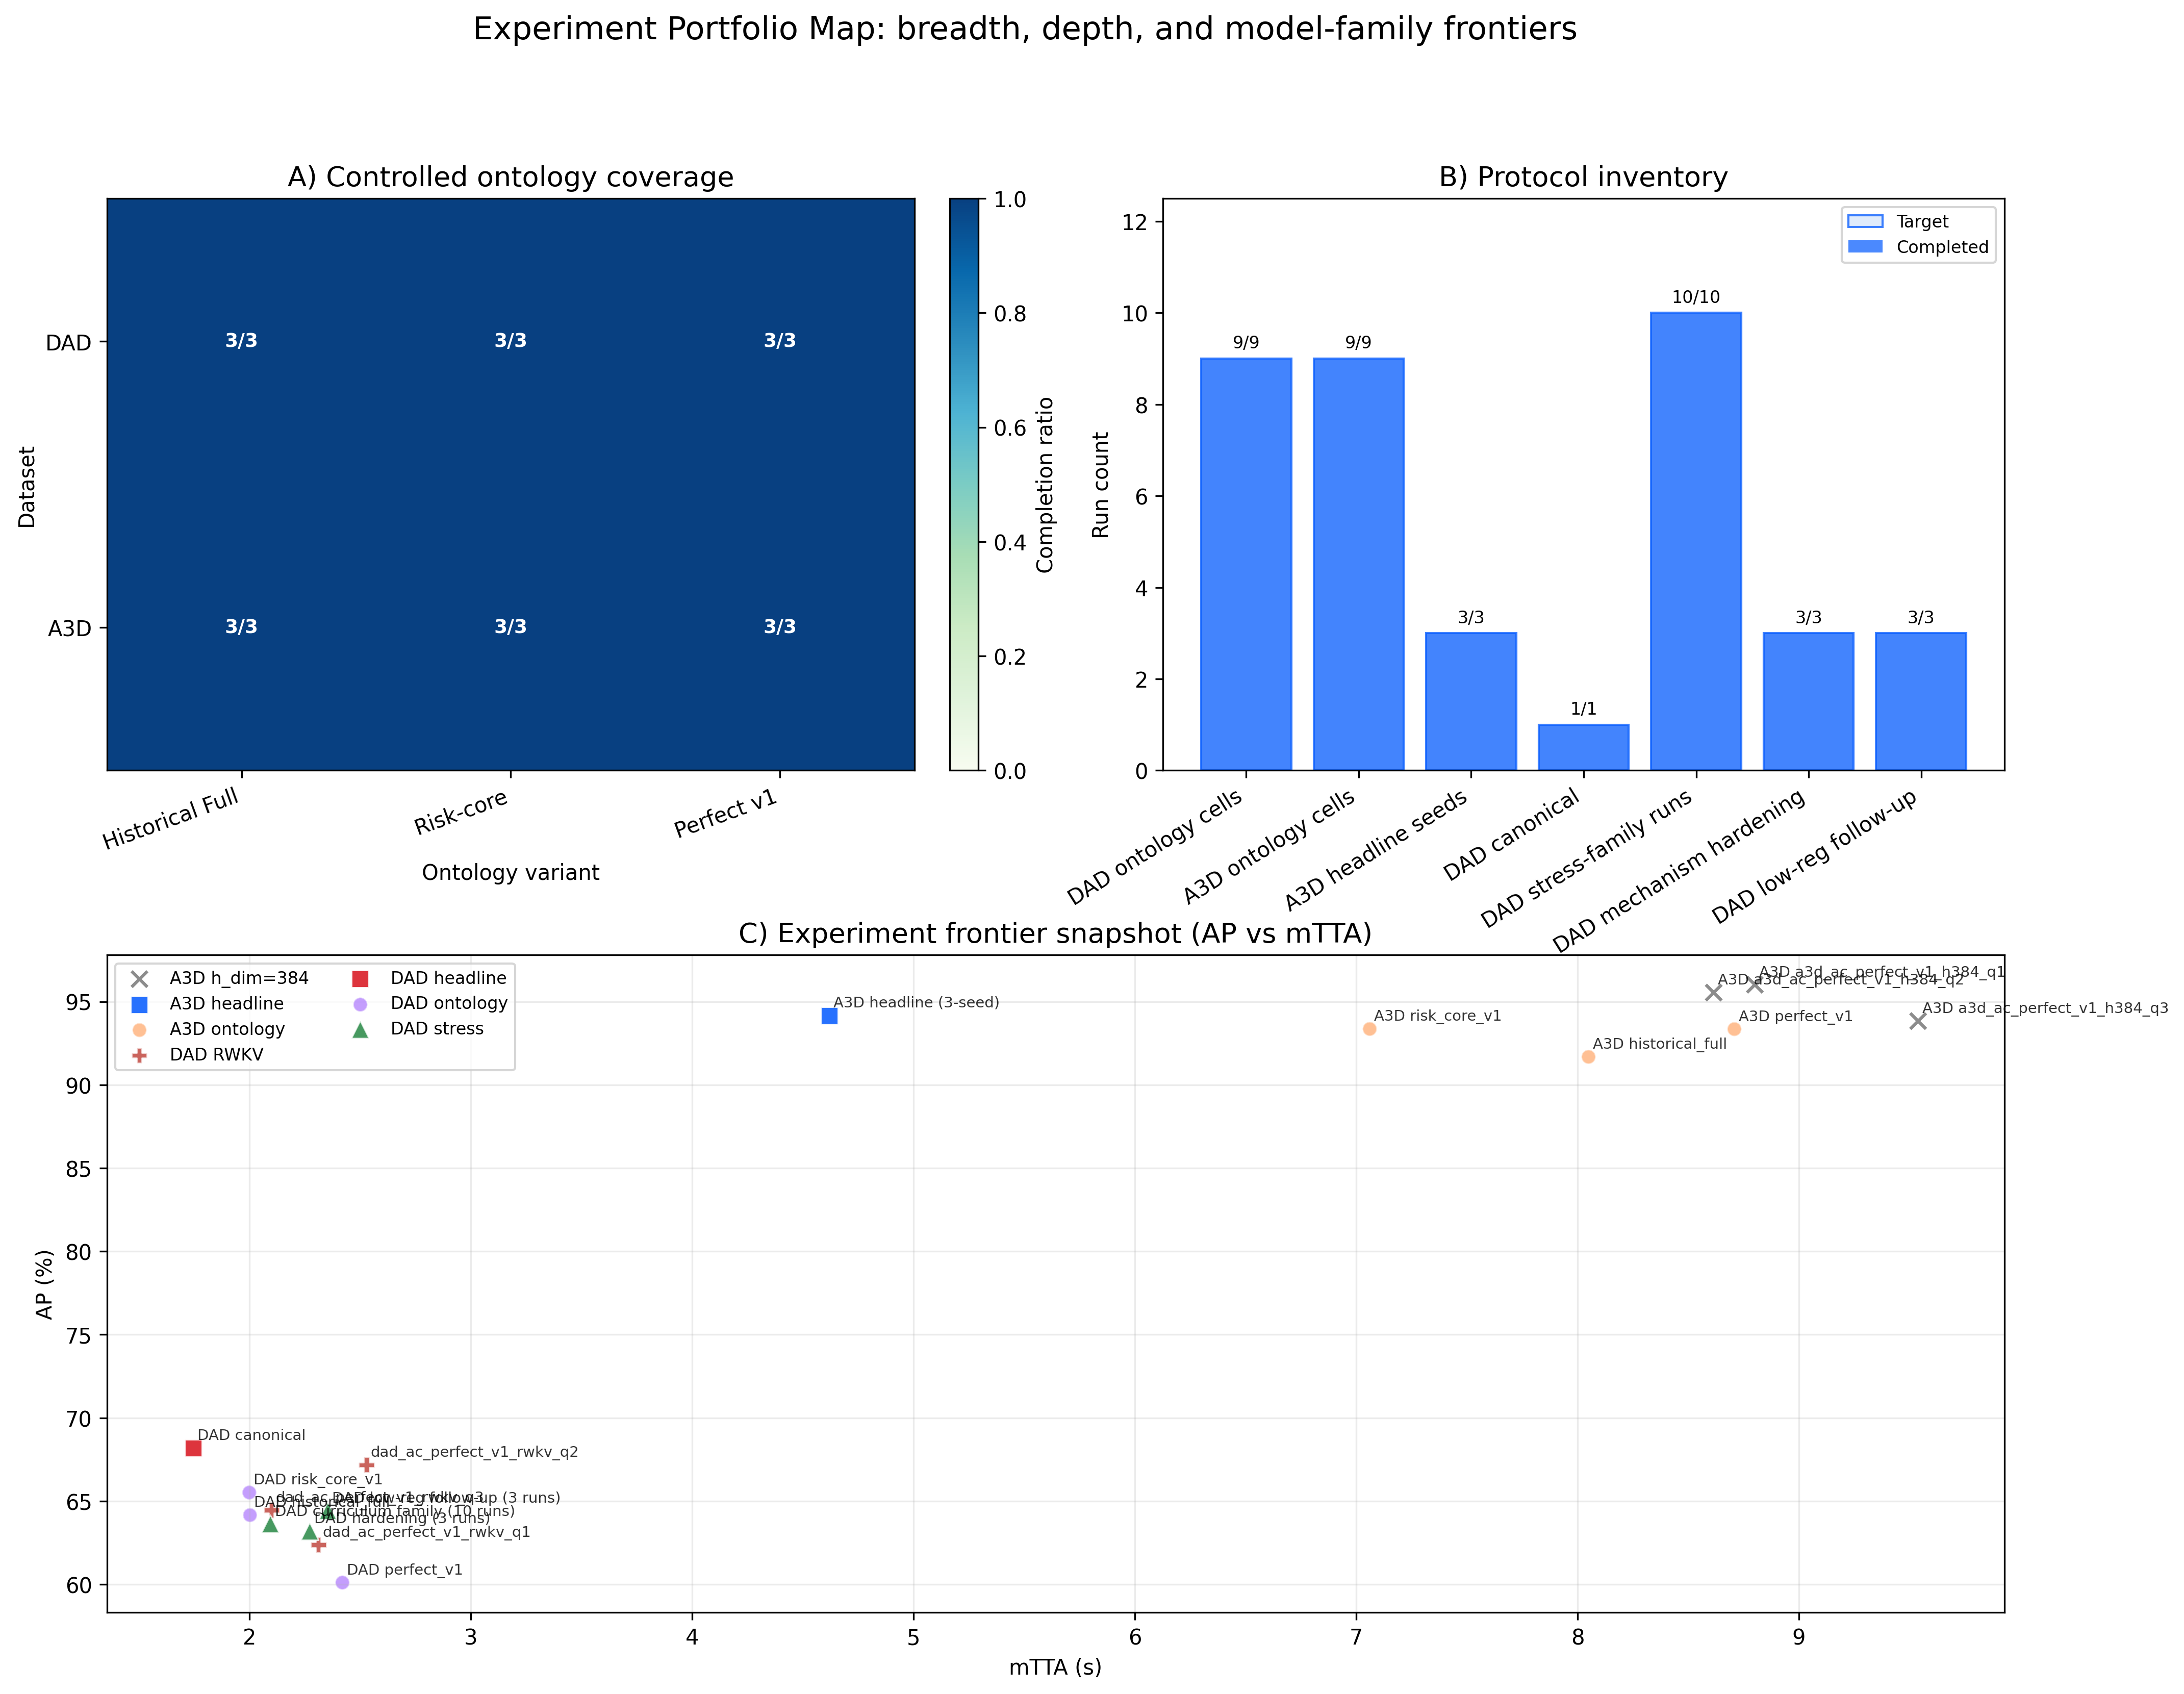
\includegraphics[width=0.98\textwidth]{../figures/insight_fig9_experiment_portfolio.pdf}
\caption{[Reading-map evidence] Experiment portfolio map used for claim-tier reading. Panel A
shows completion ratios for the controlled ontology matrix (DAD/A3D $\times$
three ontology variants). Panel B summarizes protocol depth by evidence family.
Panel C places headline, ontology, stress, and architecture-extension runs on
the same AP--mTTA plane. The figure makes execution coverage explicit without
mixing support evidence into headline claims.}
\label{fig:experiment_portfolio}
\end{figure*}
\subsection{Visual evidence upgrade: intervention gallery (support-only)}
\label{sec:intervention-gallery}
\begin{figure*}[t]
\centering
\begin{subfigure}{0.323\textwidth}
  \centering
  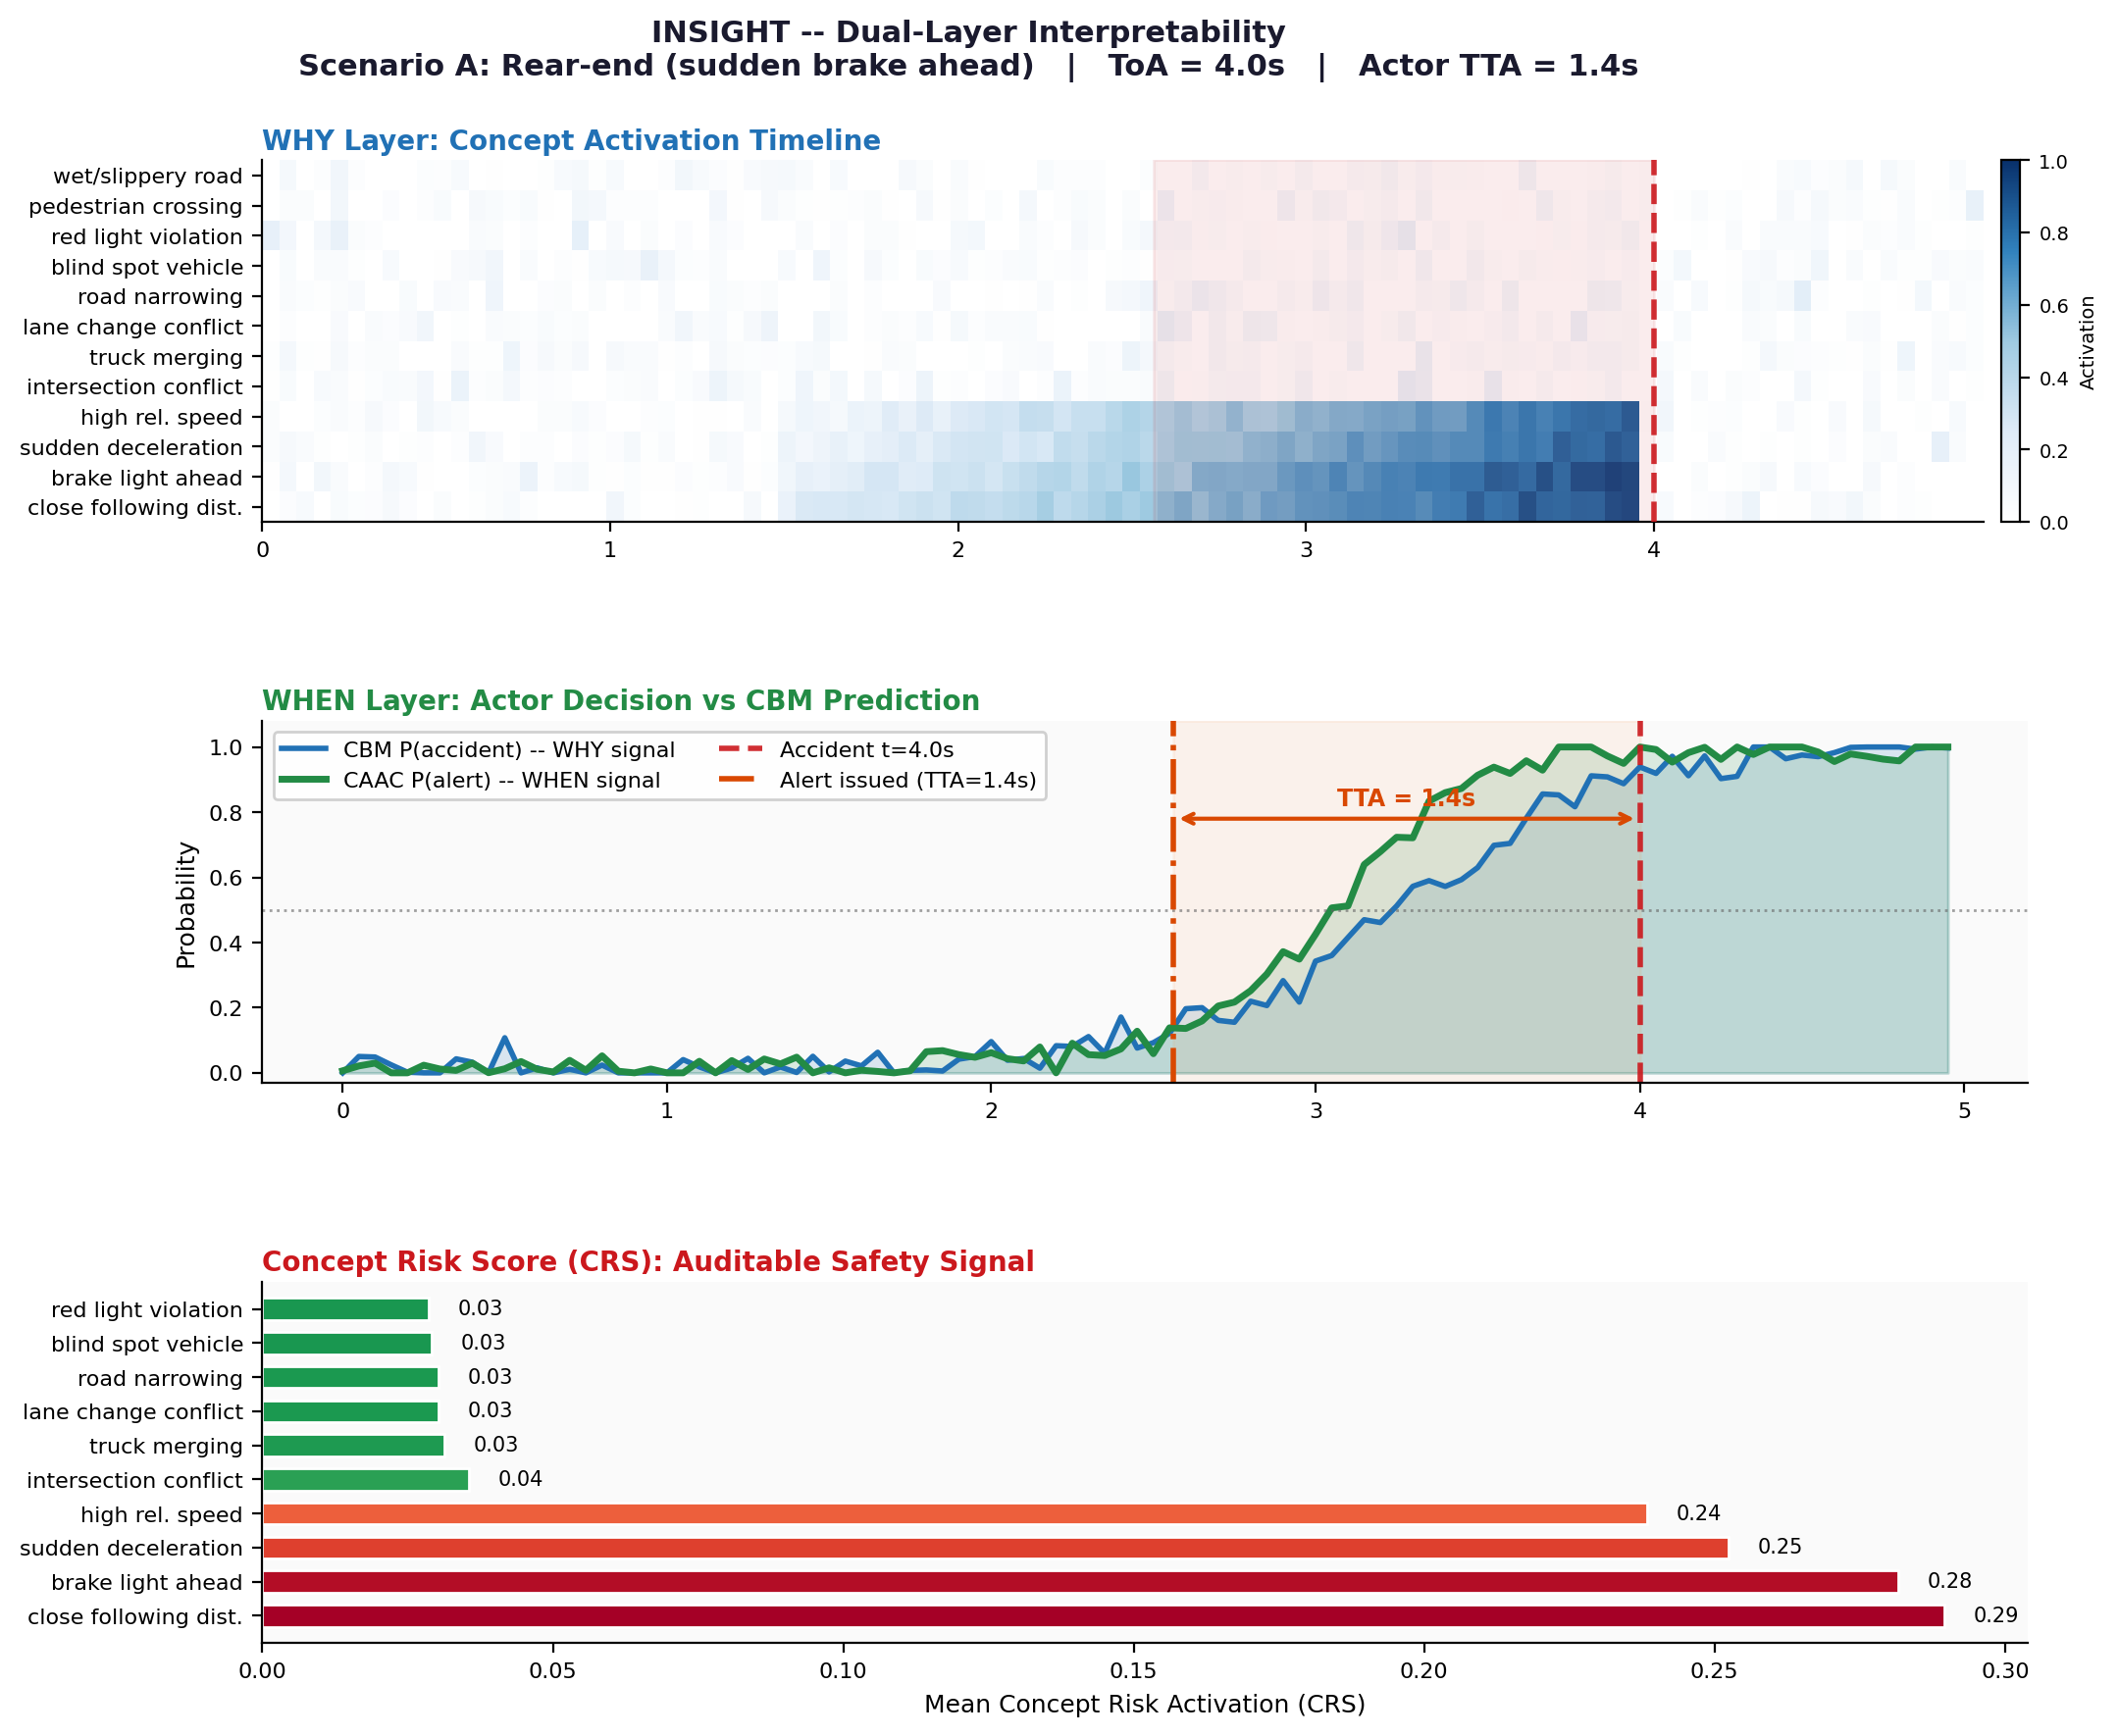
\includegraphics[width=\linewidth]{../figures/dual_interp_case1.png}
  \caption{Case 1}
\end{subfigure}
\hfill
\begin{subfigure}{0.323\textwidth}
  \centering
  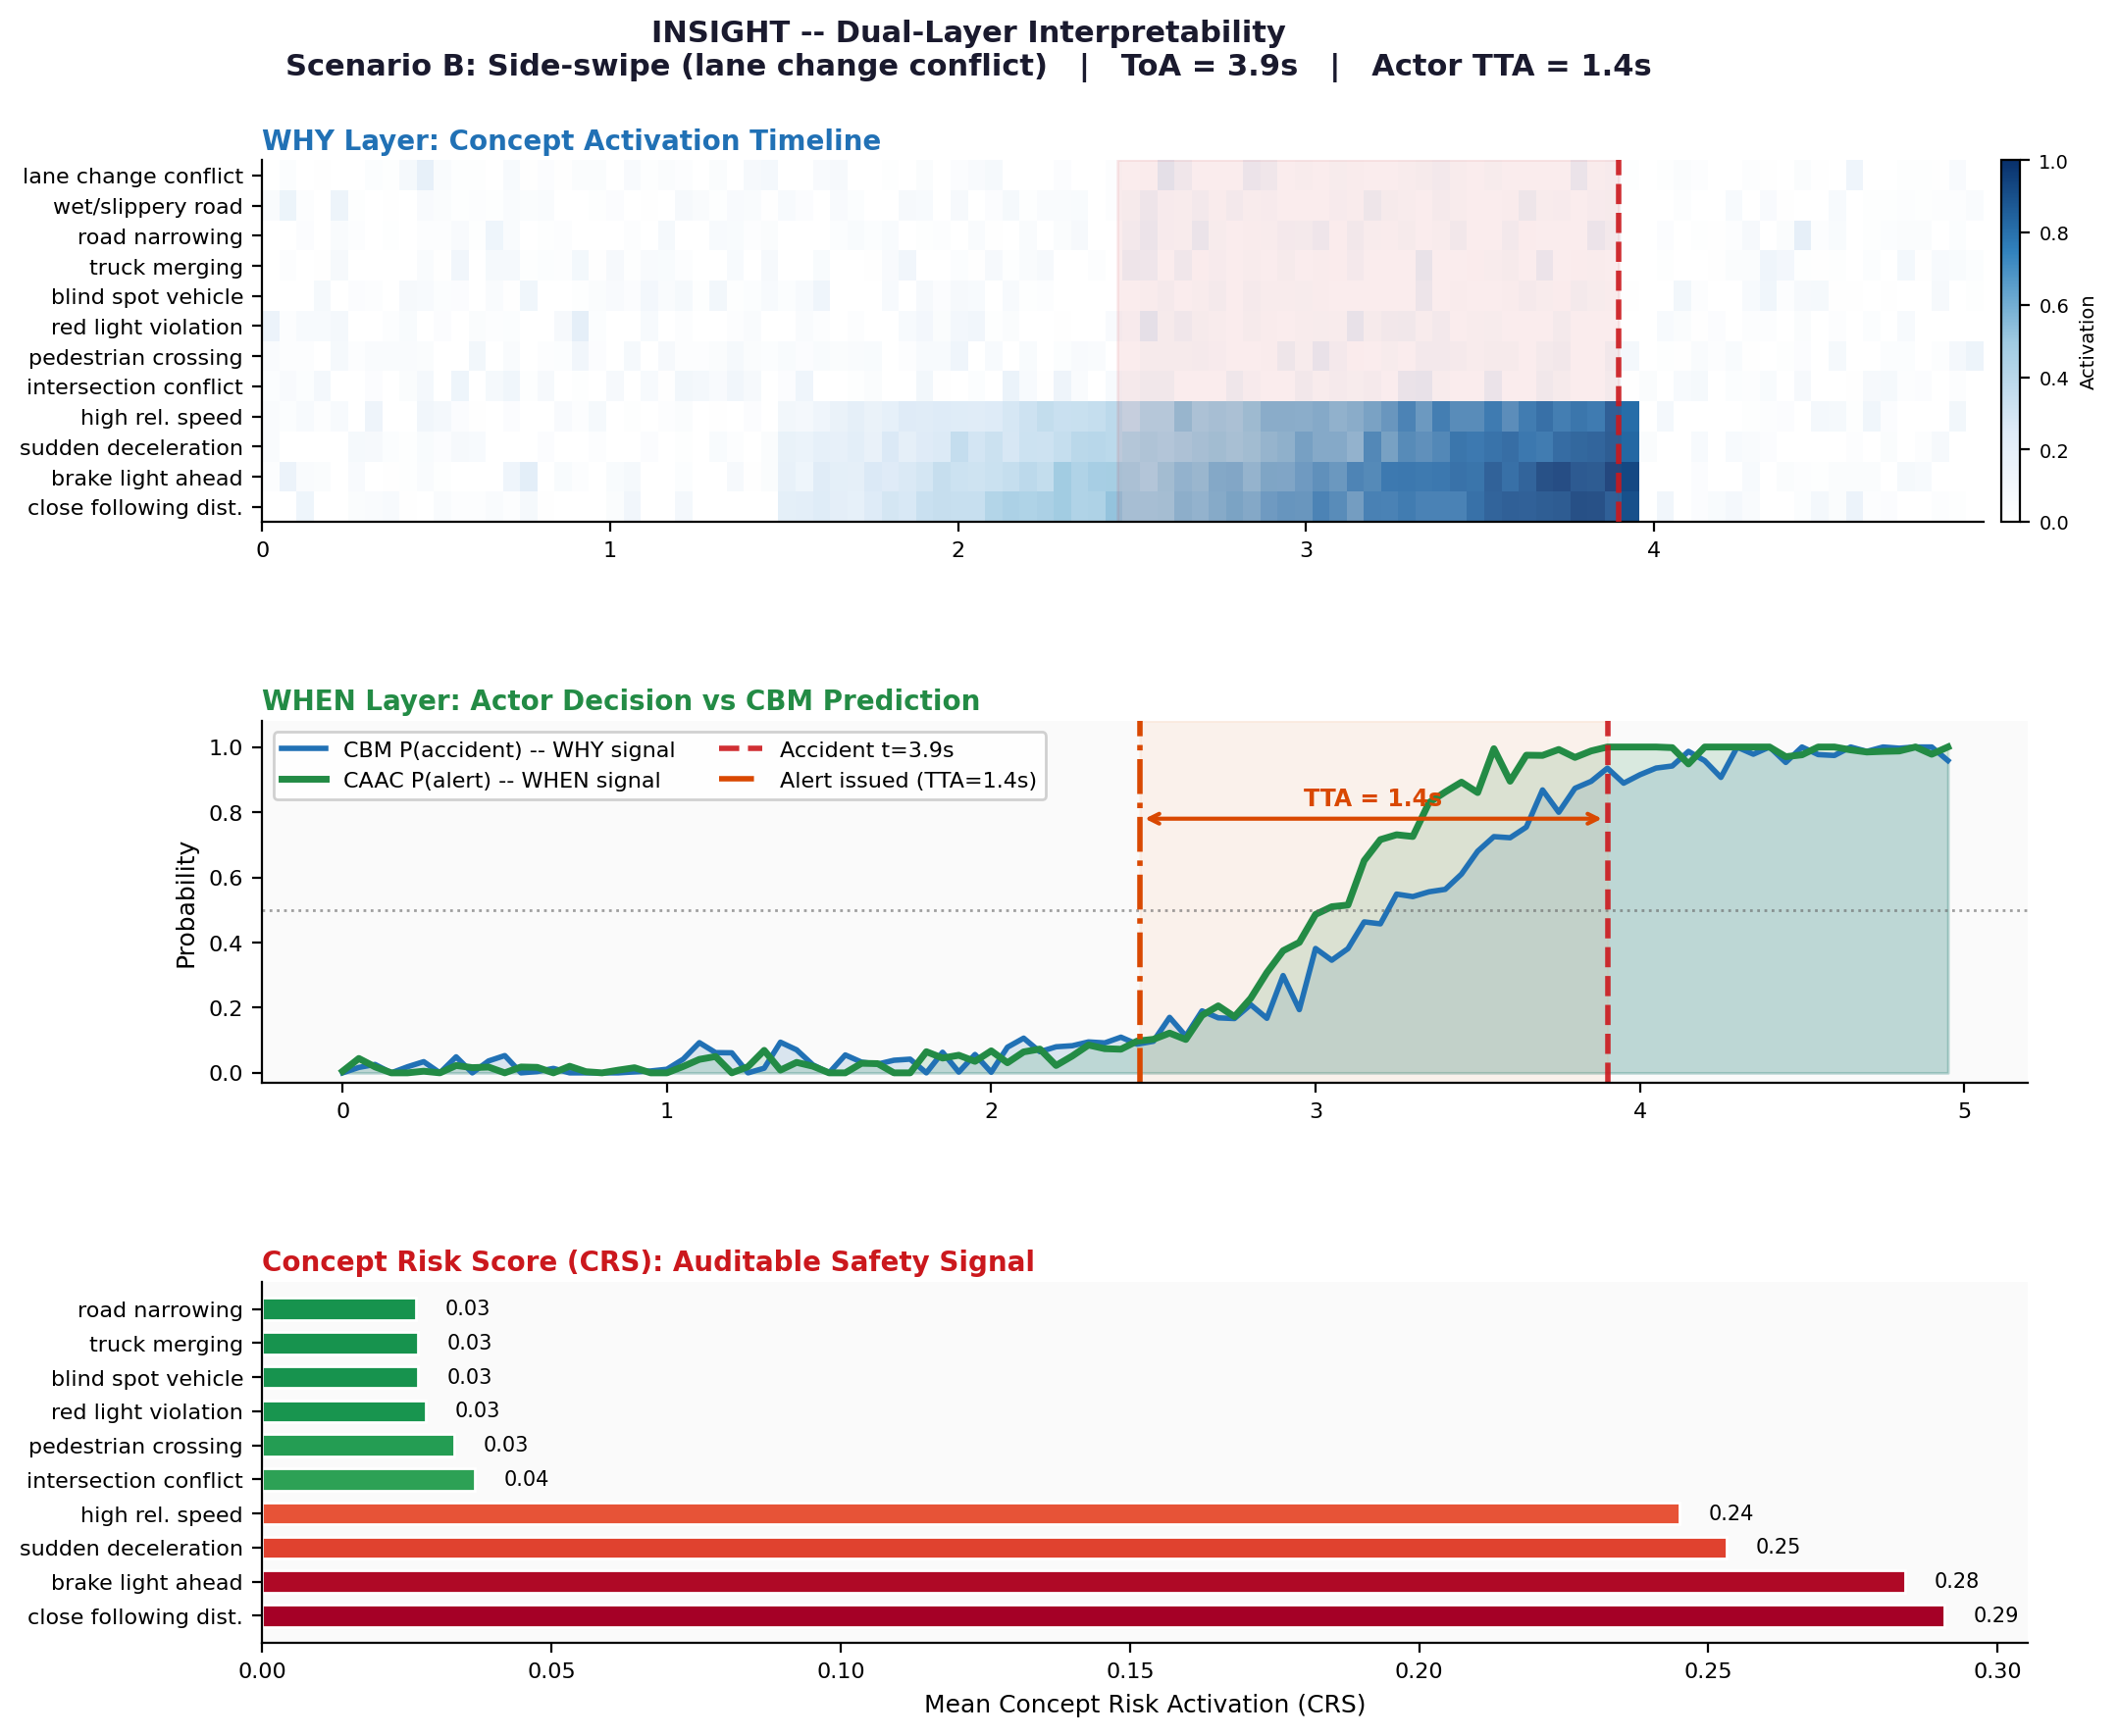
\includegraphics[width=\linewidth]{../figures/dual_interp_case2.png}
  \caption{Case 2}
\end{subfigure}
\hfill
\begin{subfigure}{0.323\textwidth}
  \centering
  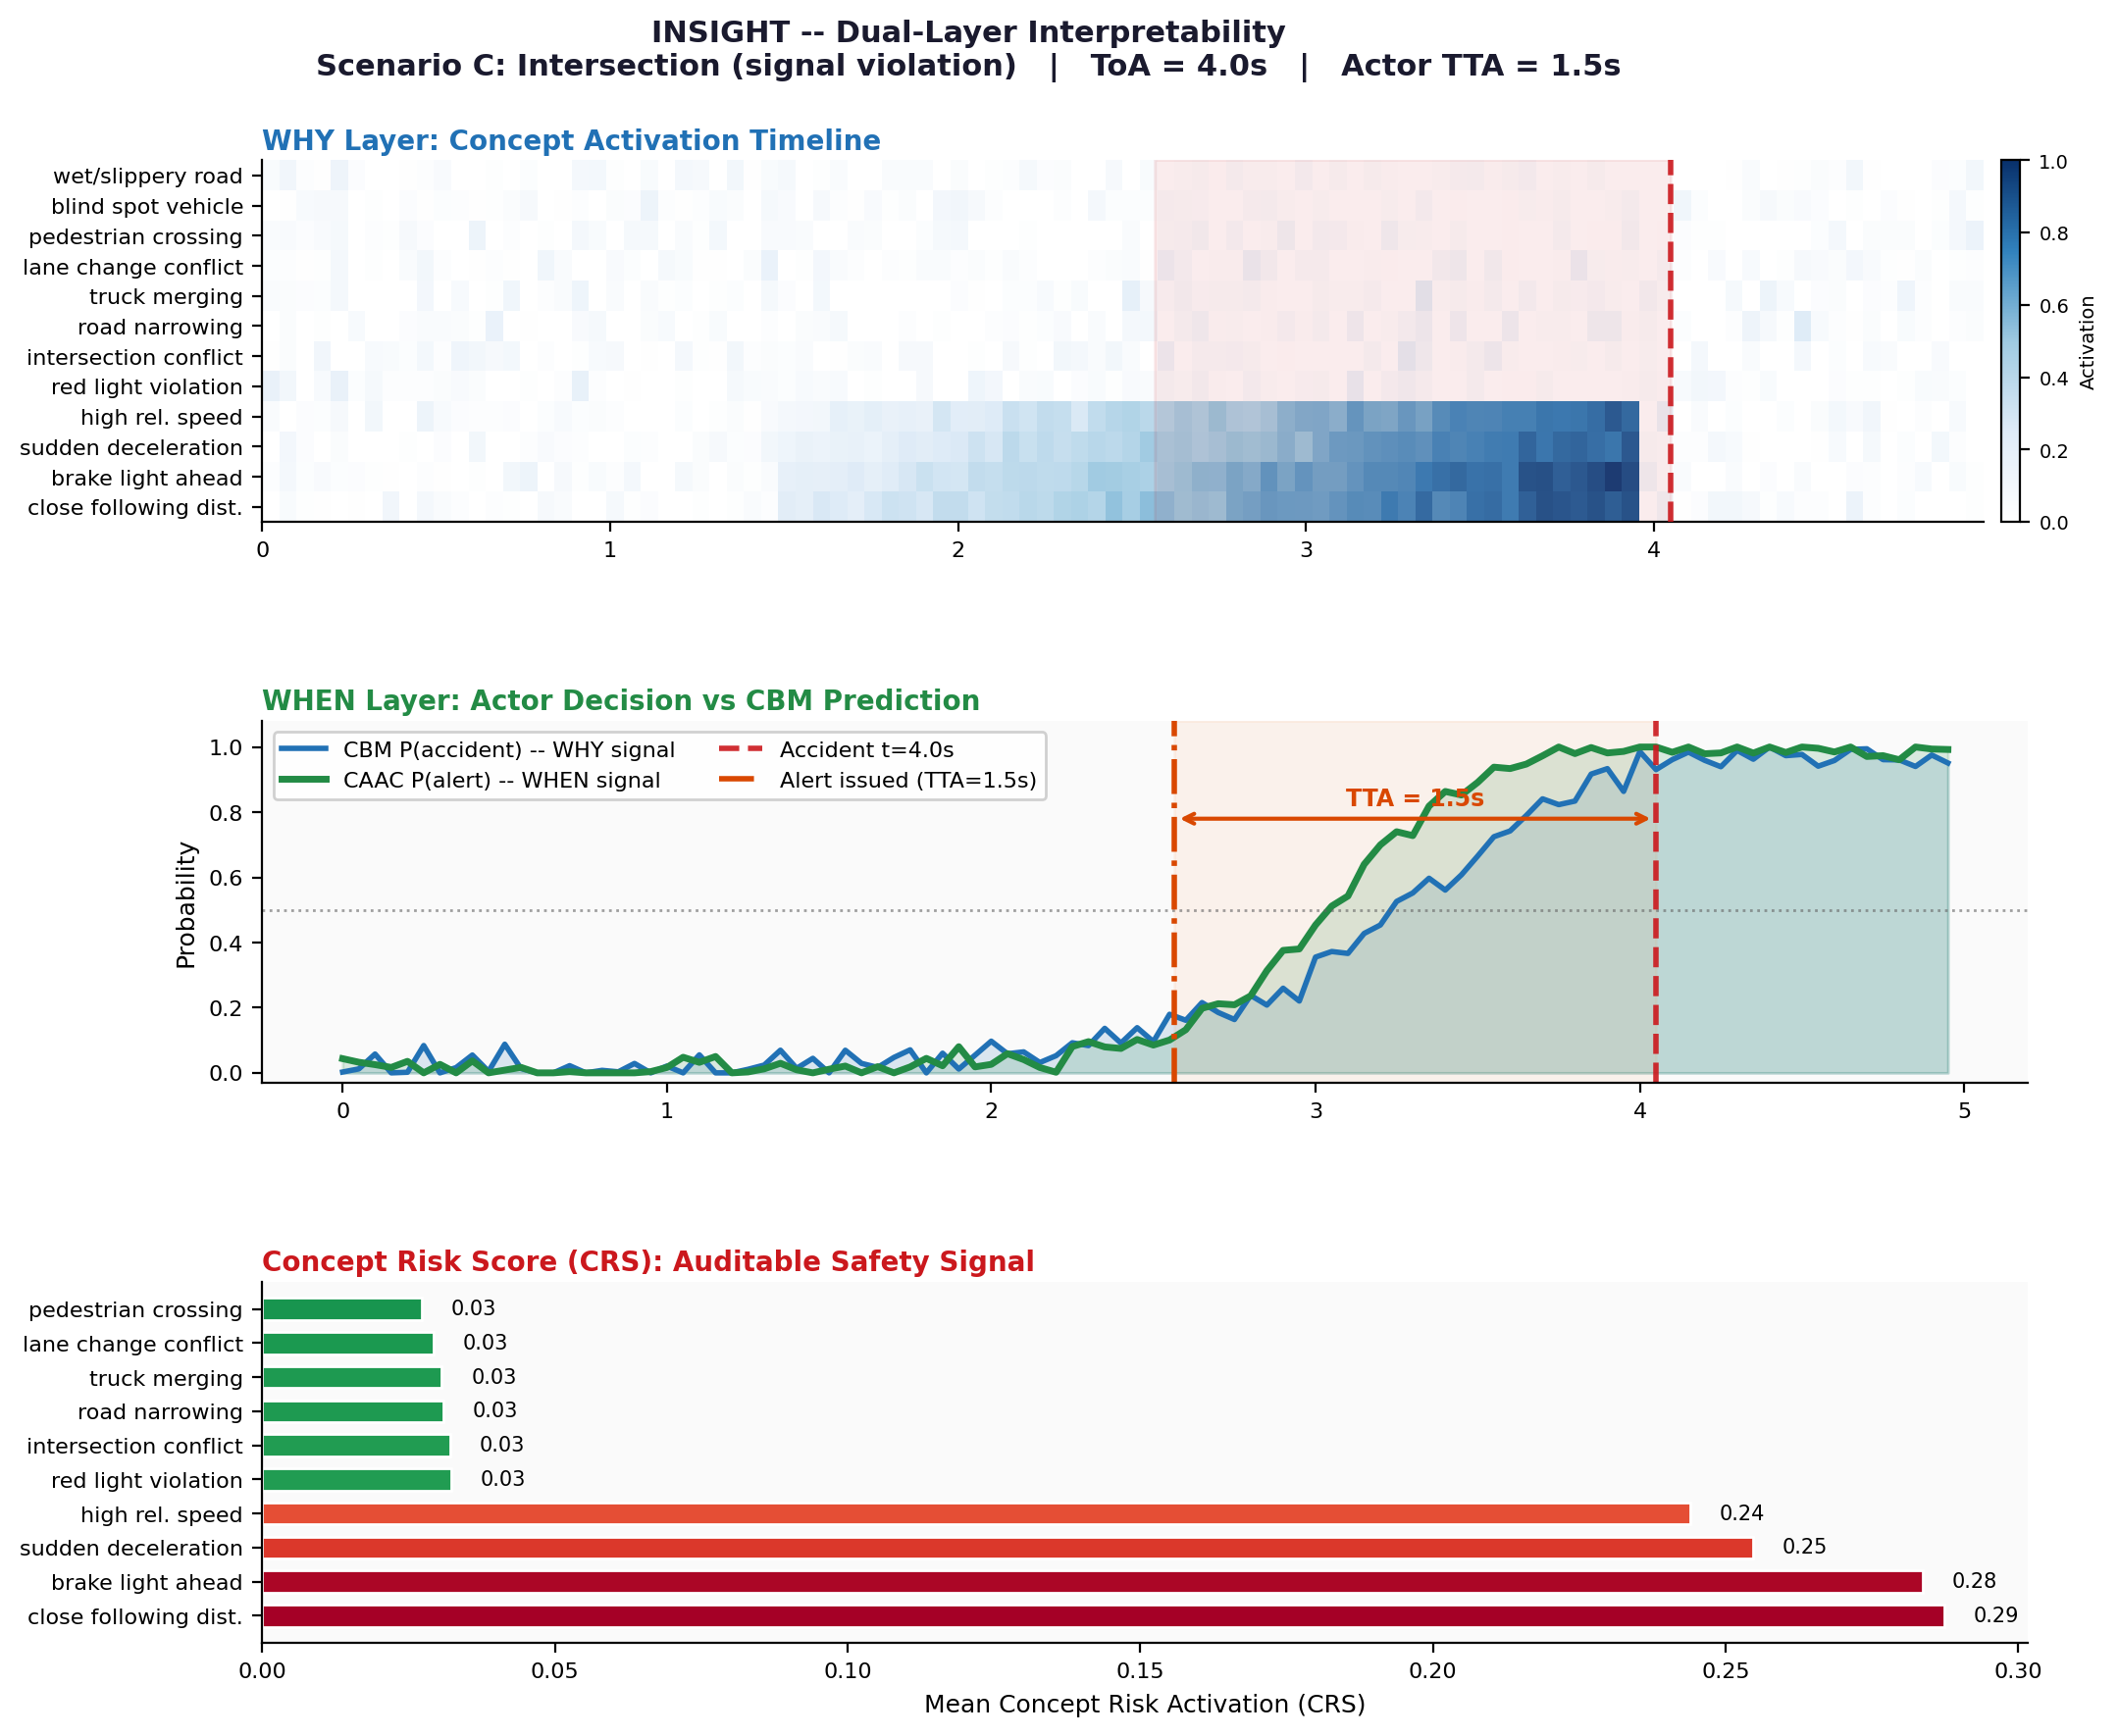
\includegraphics[width=\linewidth]{../figures/dual_interp_case3.png}
  \caption{Case 3}
\end{subfigure}
\caption{Support-only intervention gallery. The three paired DAD cases show how concept edits
alter activation trajectories under the same ontology protocol and where timing effects
do and do not change direction. It is intended as mechanistic intuition, not a headline result.}
\label{fig:intervention_gallery}
\end{figure*}

\begin{figure*}[t]
\centering
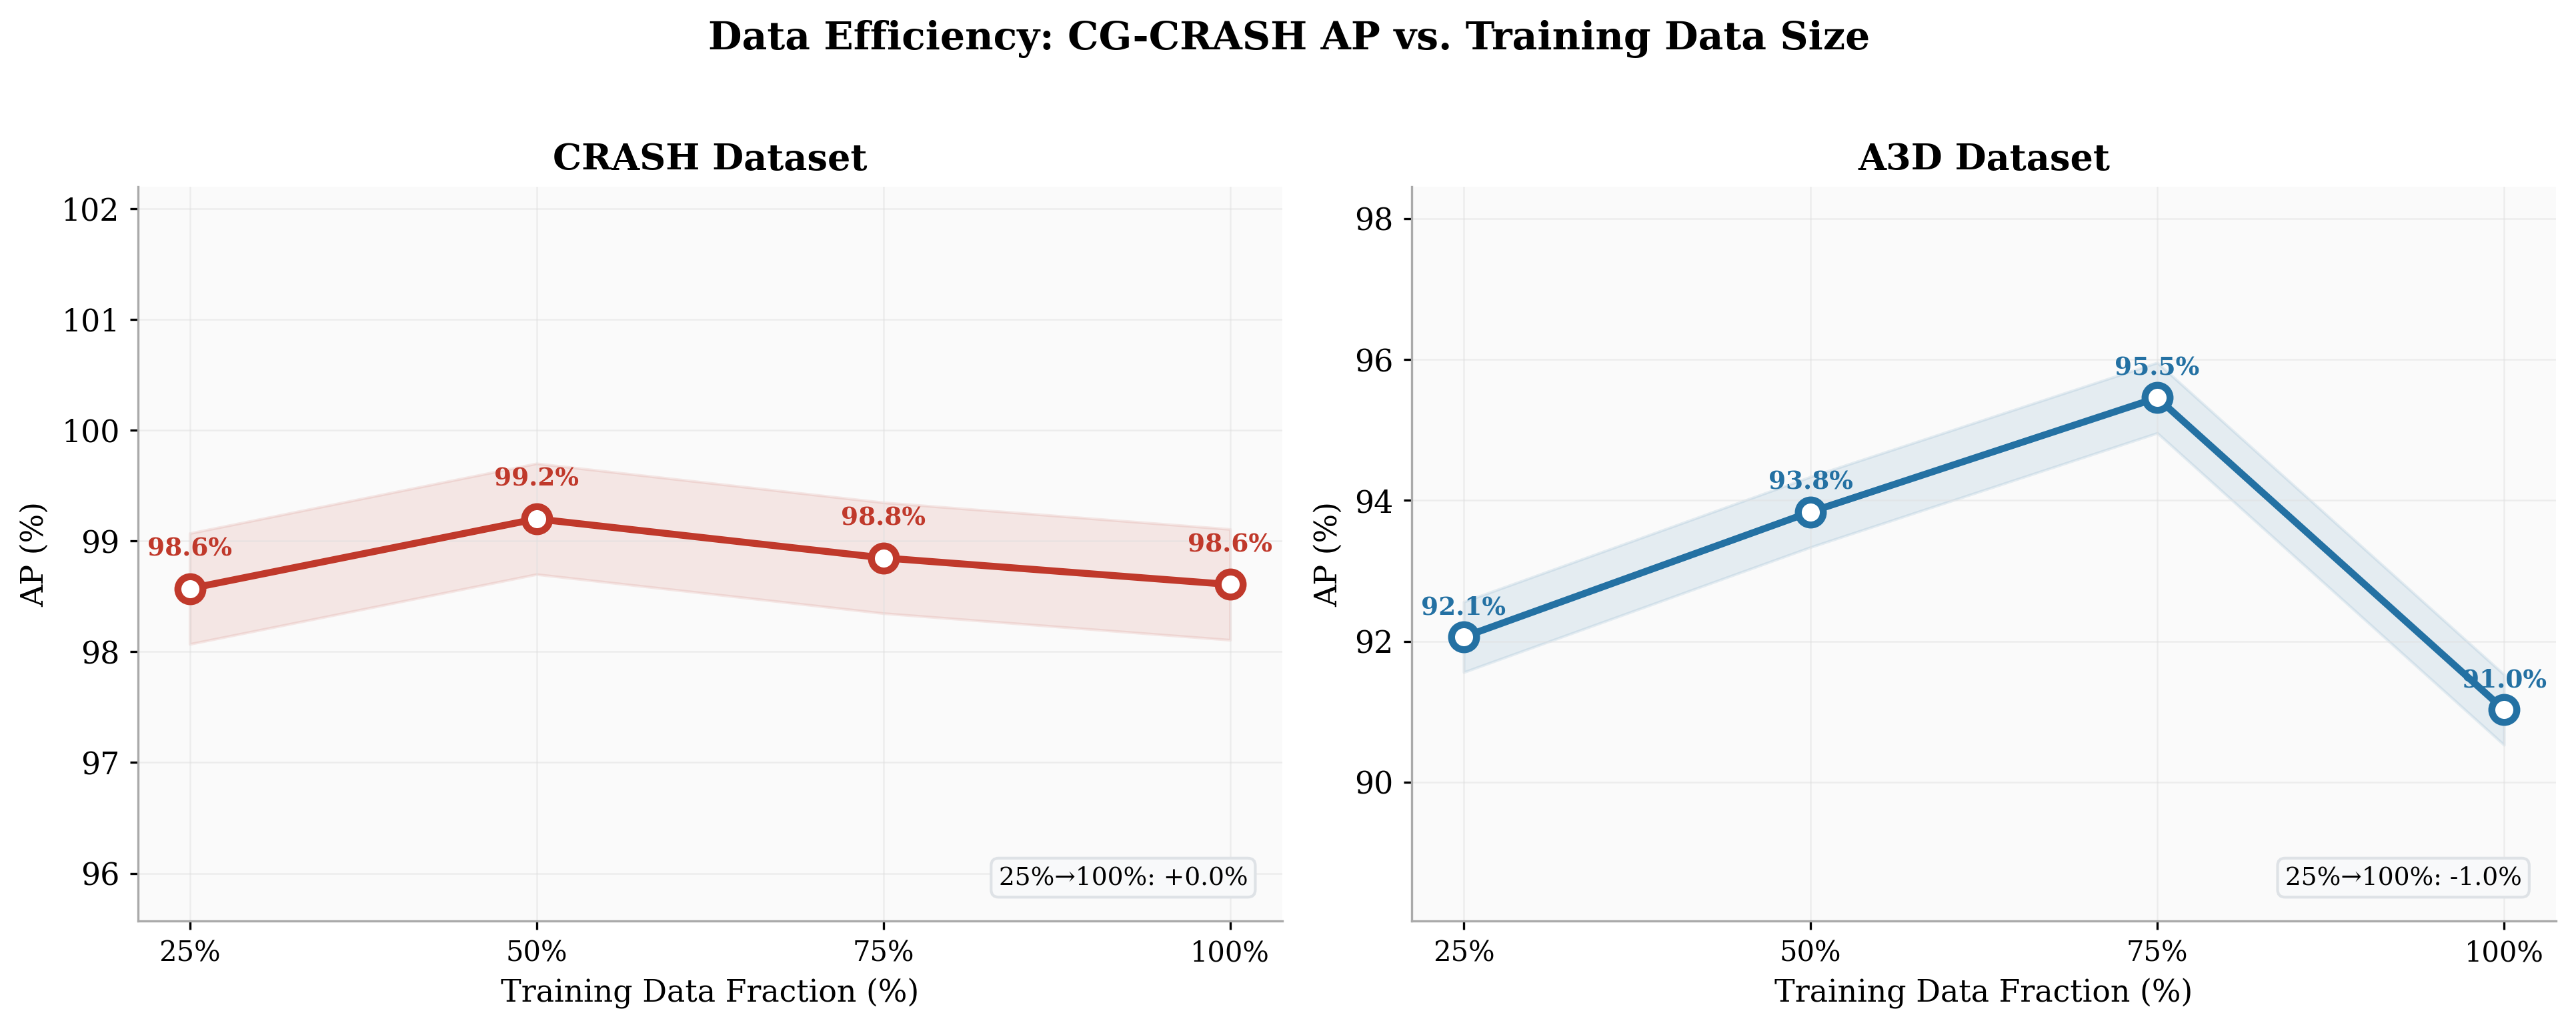
\includegraphics[width=0.98\textwidth]{../figures/insight_fig7_data_efficiency.pdf}
\caption{Cross-regime robustness check from data-fraction probes on CRASH, DAD, and
A3D. Broader dataset behavior is compared in the same protocol family, while
headline claims remain scoped by the tabulated results.}
\label{fig:data_efficiency}
\end{figure*}

\begin{figure*}[t]
  \centering
  \begin{subfigure}{0.495\textwidth}
    \centering
    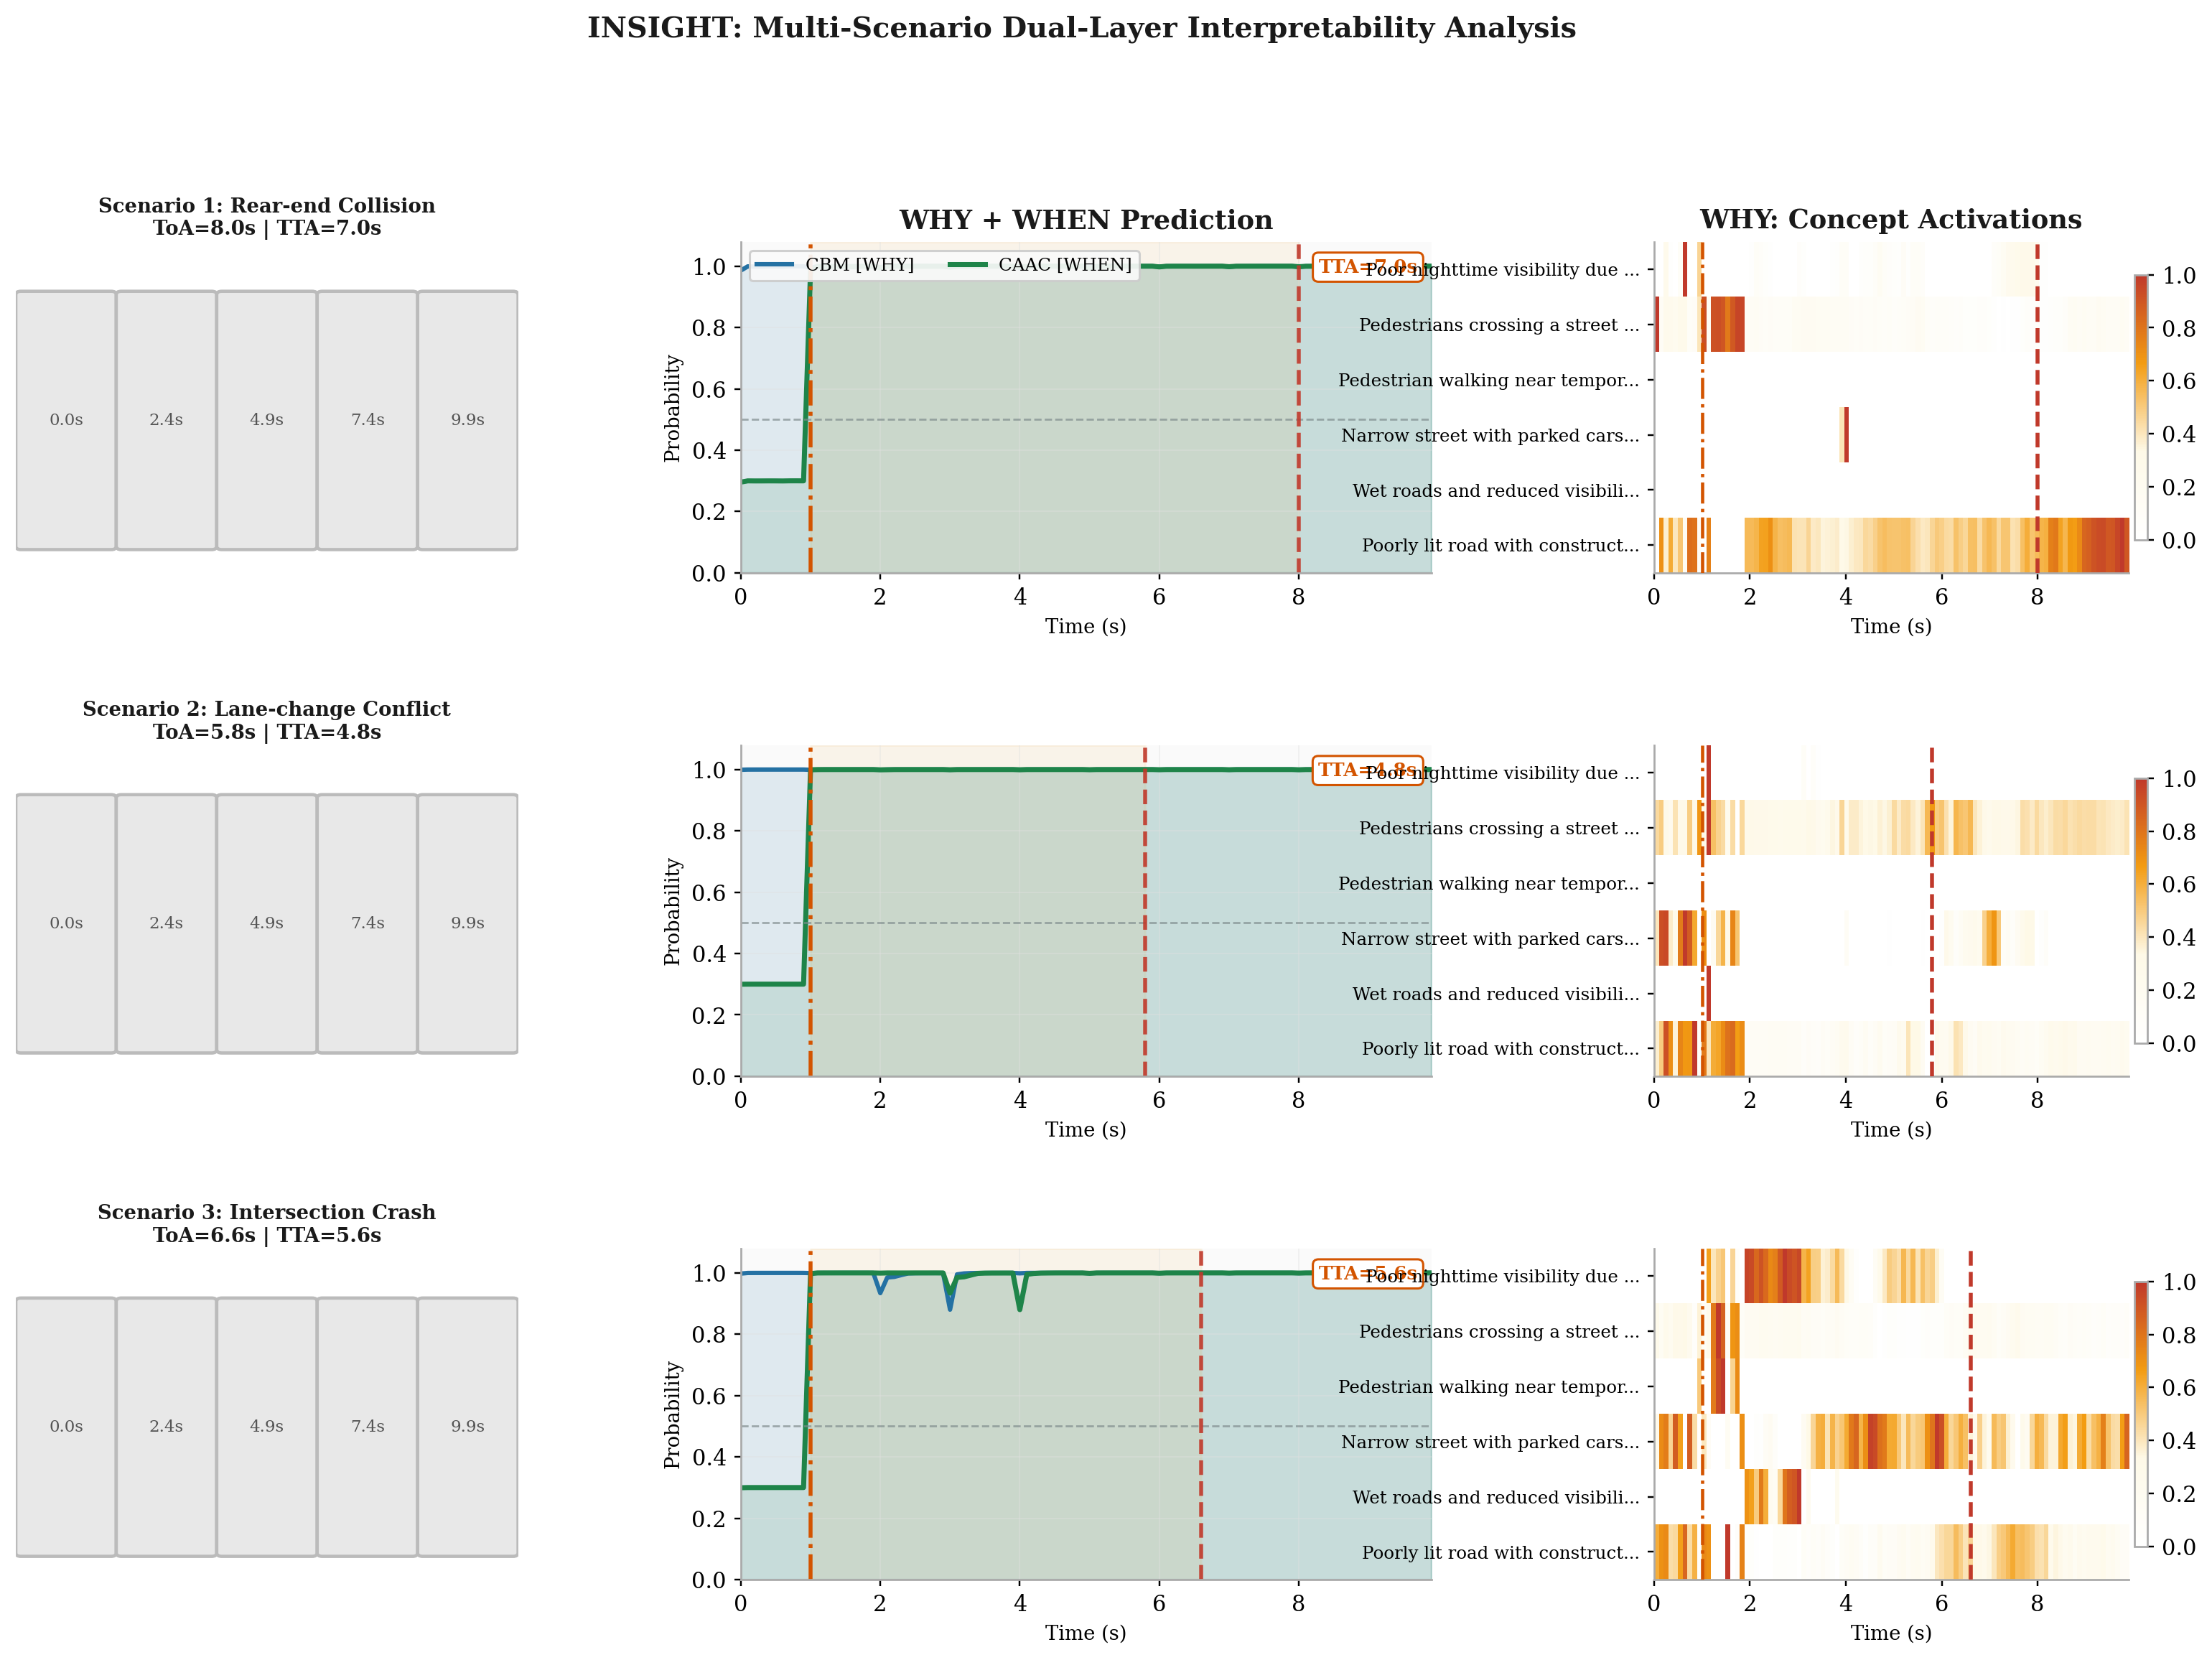
\includegraphics[width=\linewidth]{../figures/insight_fig2_multi_a3d.png}
    \caption{A3D representative trajectory}
    \label{fig:qual_case_a3d}
  \end{subfigure}
  \hfill
  \begin{subfigure}{0.495\textwidth}
    \centering
    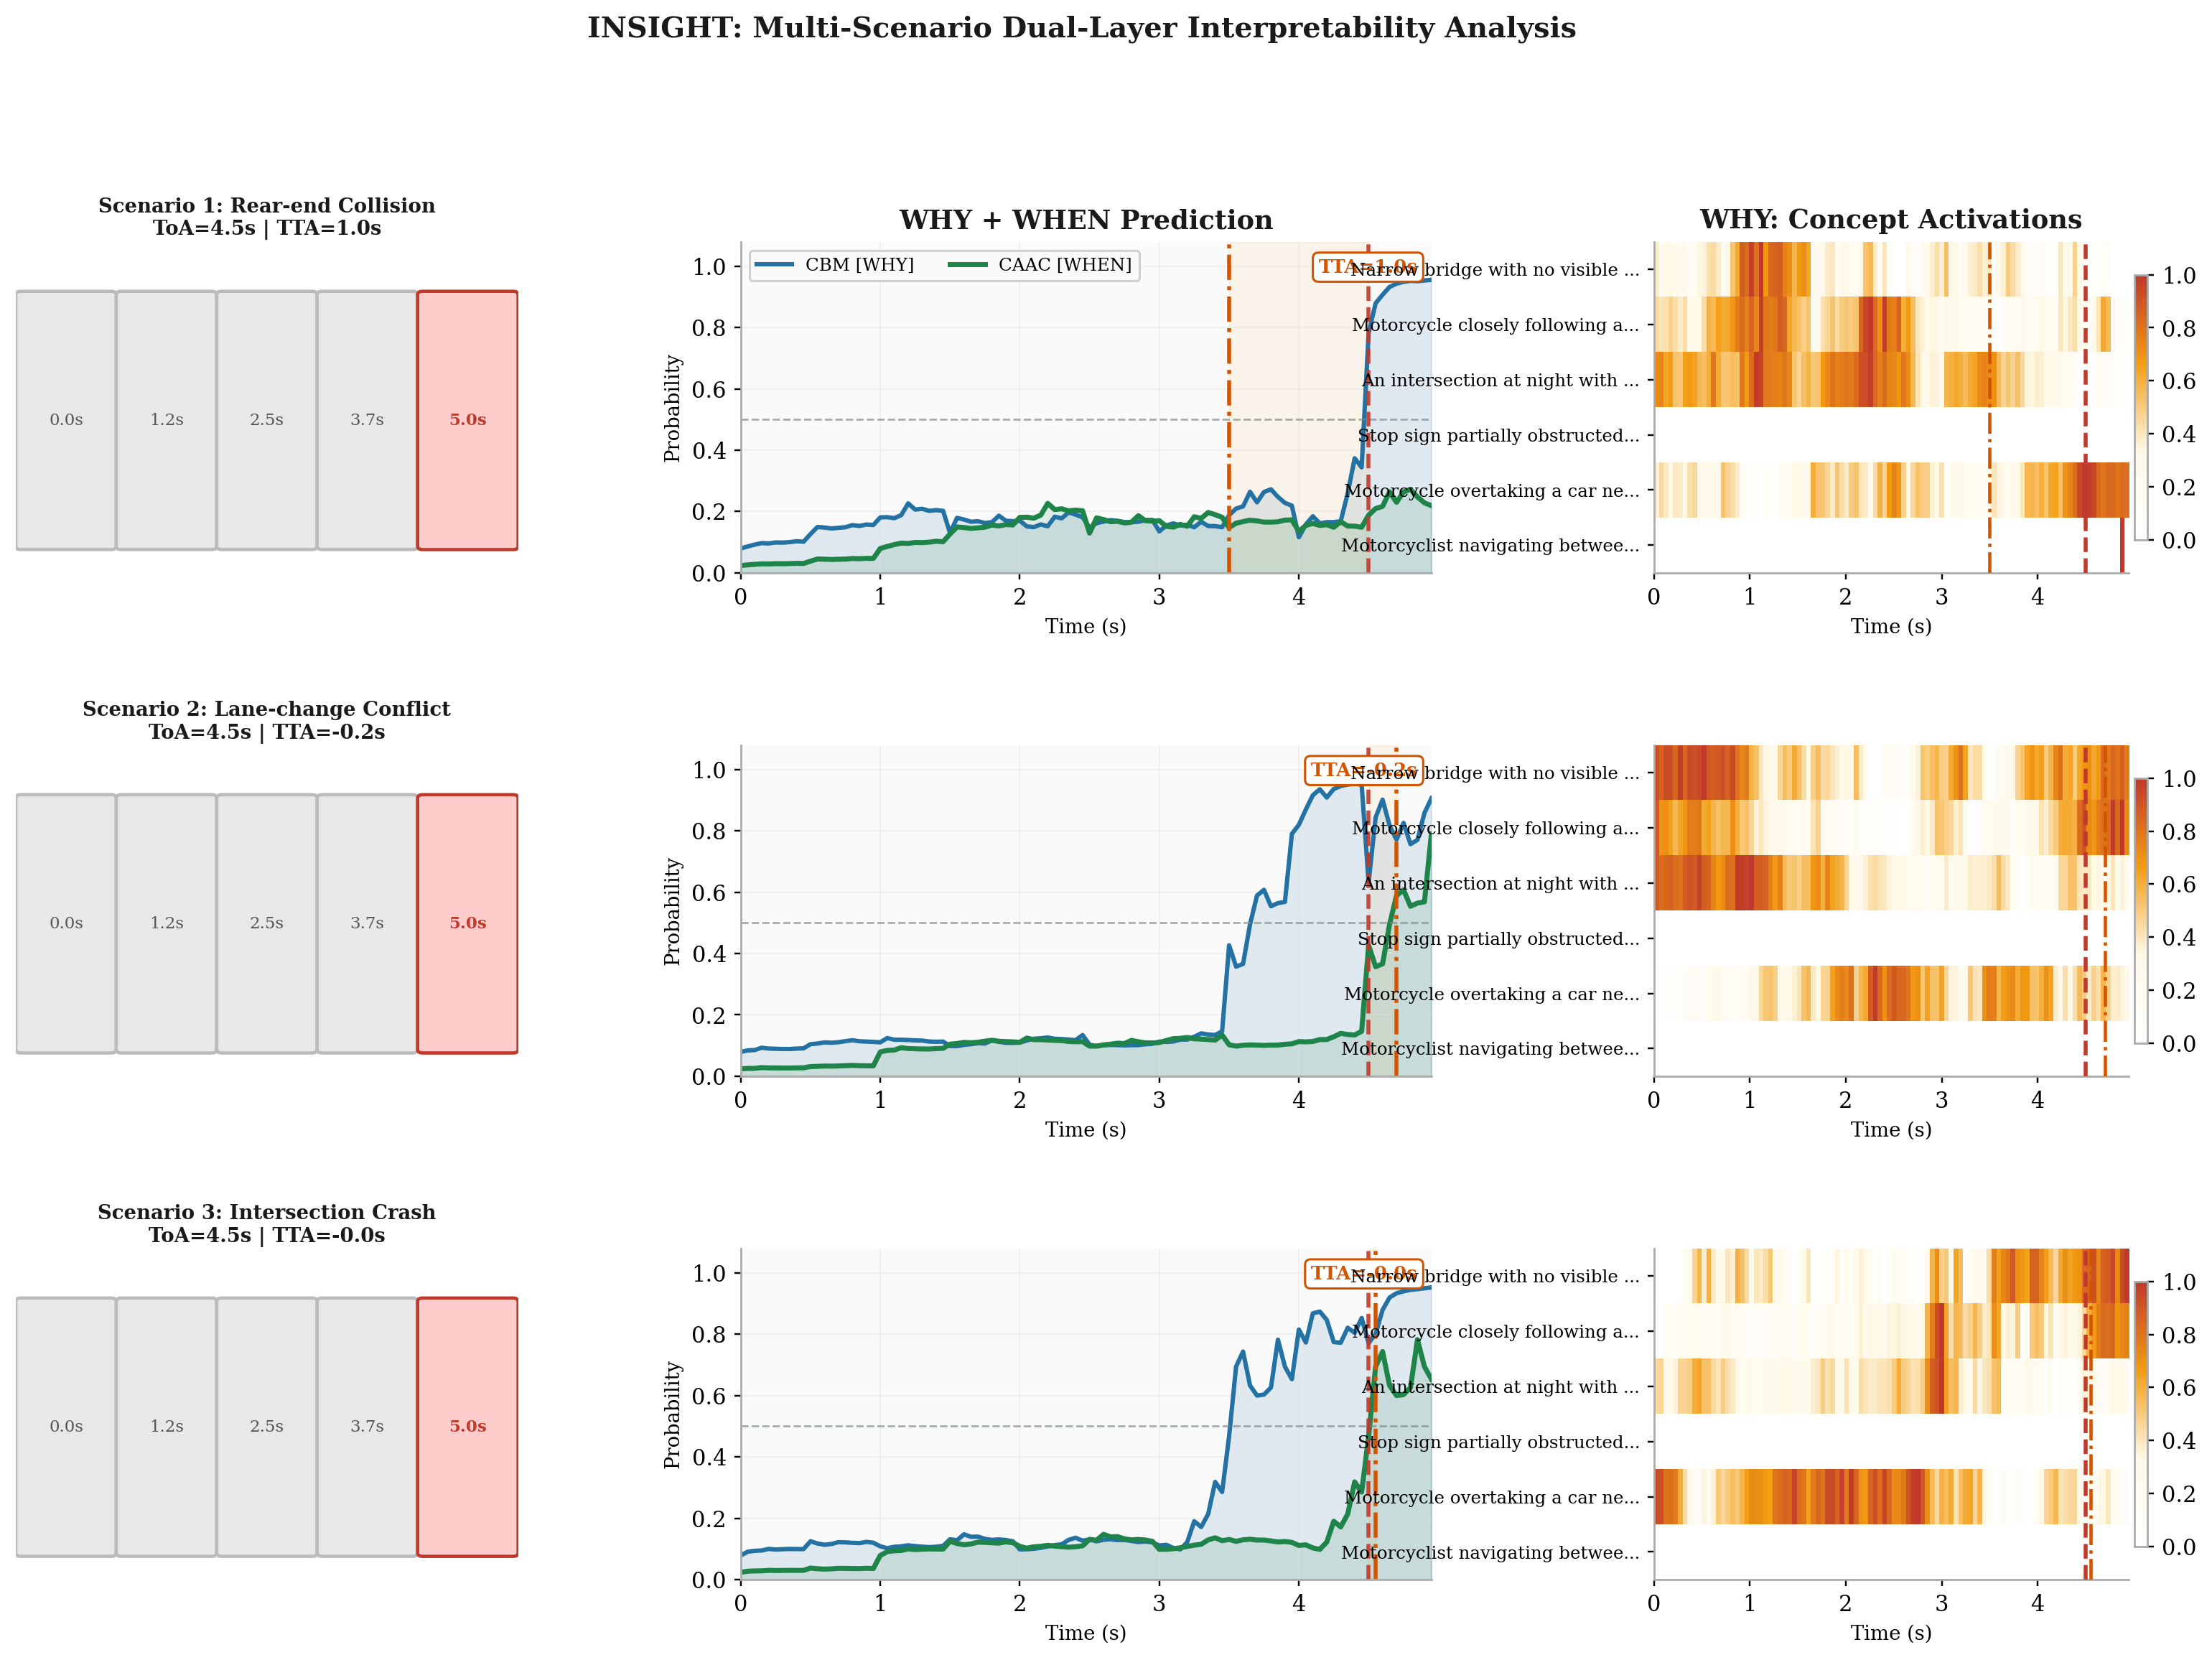
\includegraphics[width=\linewidth]{../figures/insight_fig2_multi_dad.png}
    \caption{DAD representative trajectory}
    \label{fig:qual_case_dad}
  \end{subfigure}
  \caption{Qualitative comparison of representative semantic traces. The two
  datasets show the same interface in different stress regimes: A3D exposes longer,
  progressively unfolding precursor patterns, while DAD is shorter and noisier.
  The paper uses these in-place visual checks only as intuition support; headline
  claims still use the protocol-separated quantitative blocks.}
  \label{fig:qual_case_stress}
\end{figure*}

\begin{figure*}[t]
  \centering
  \begin{subfigure}{0.495\textwidth}
    \centering
    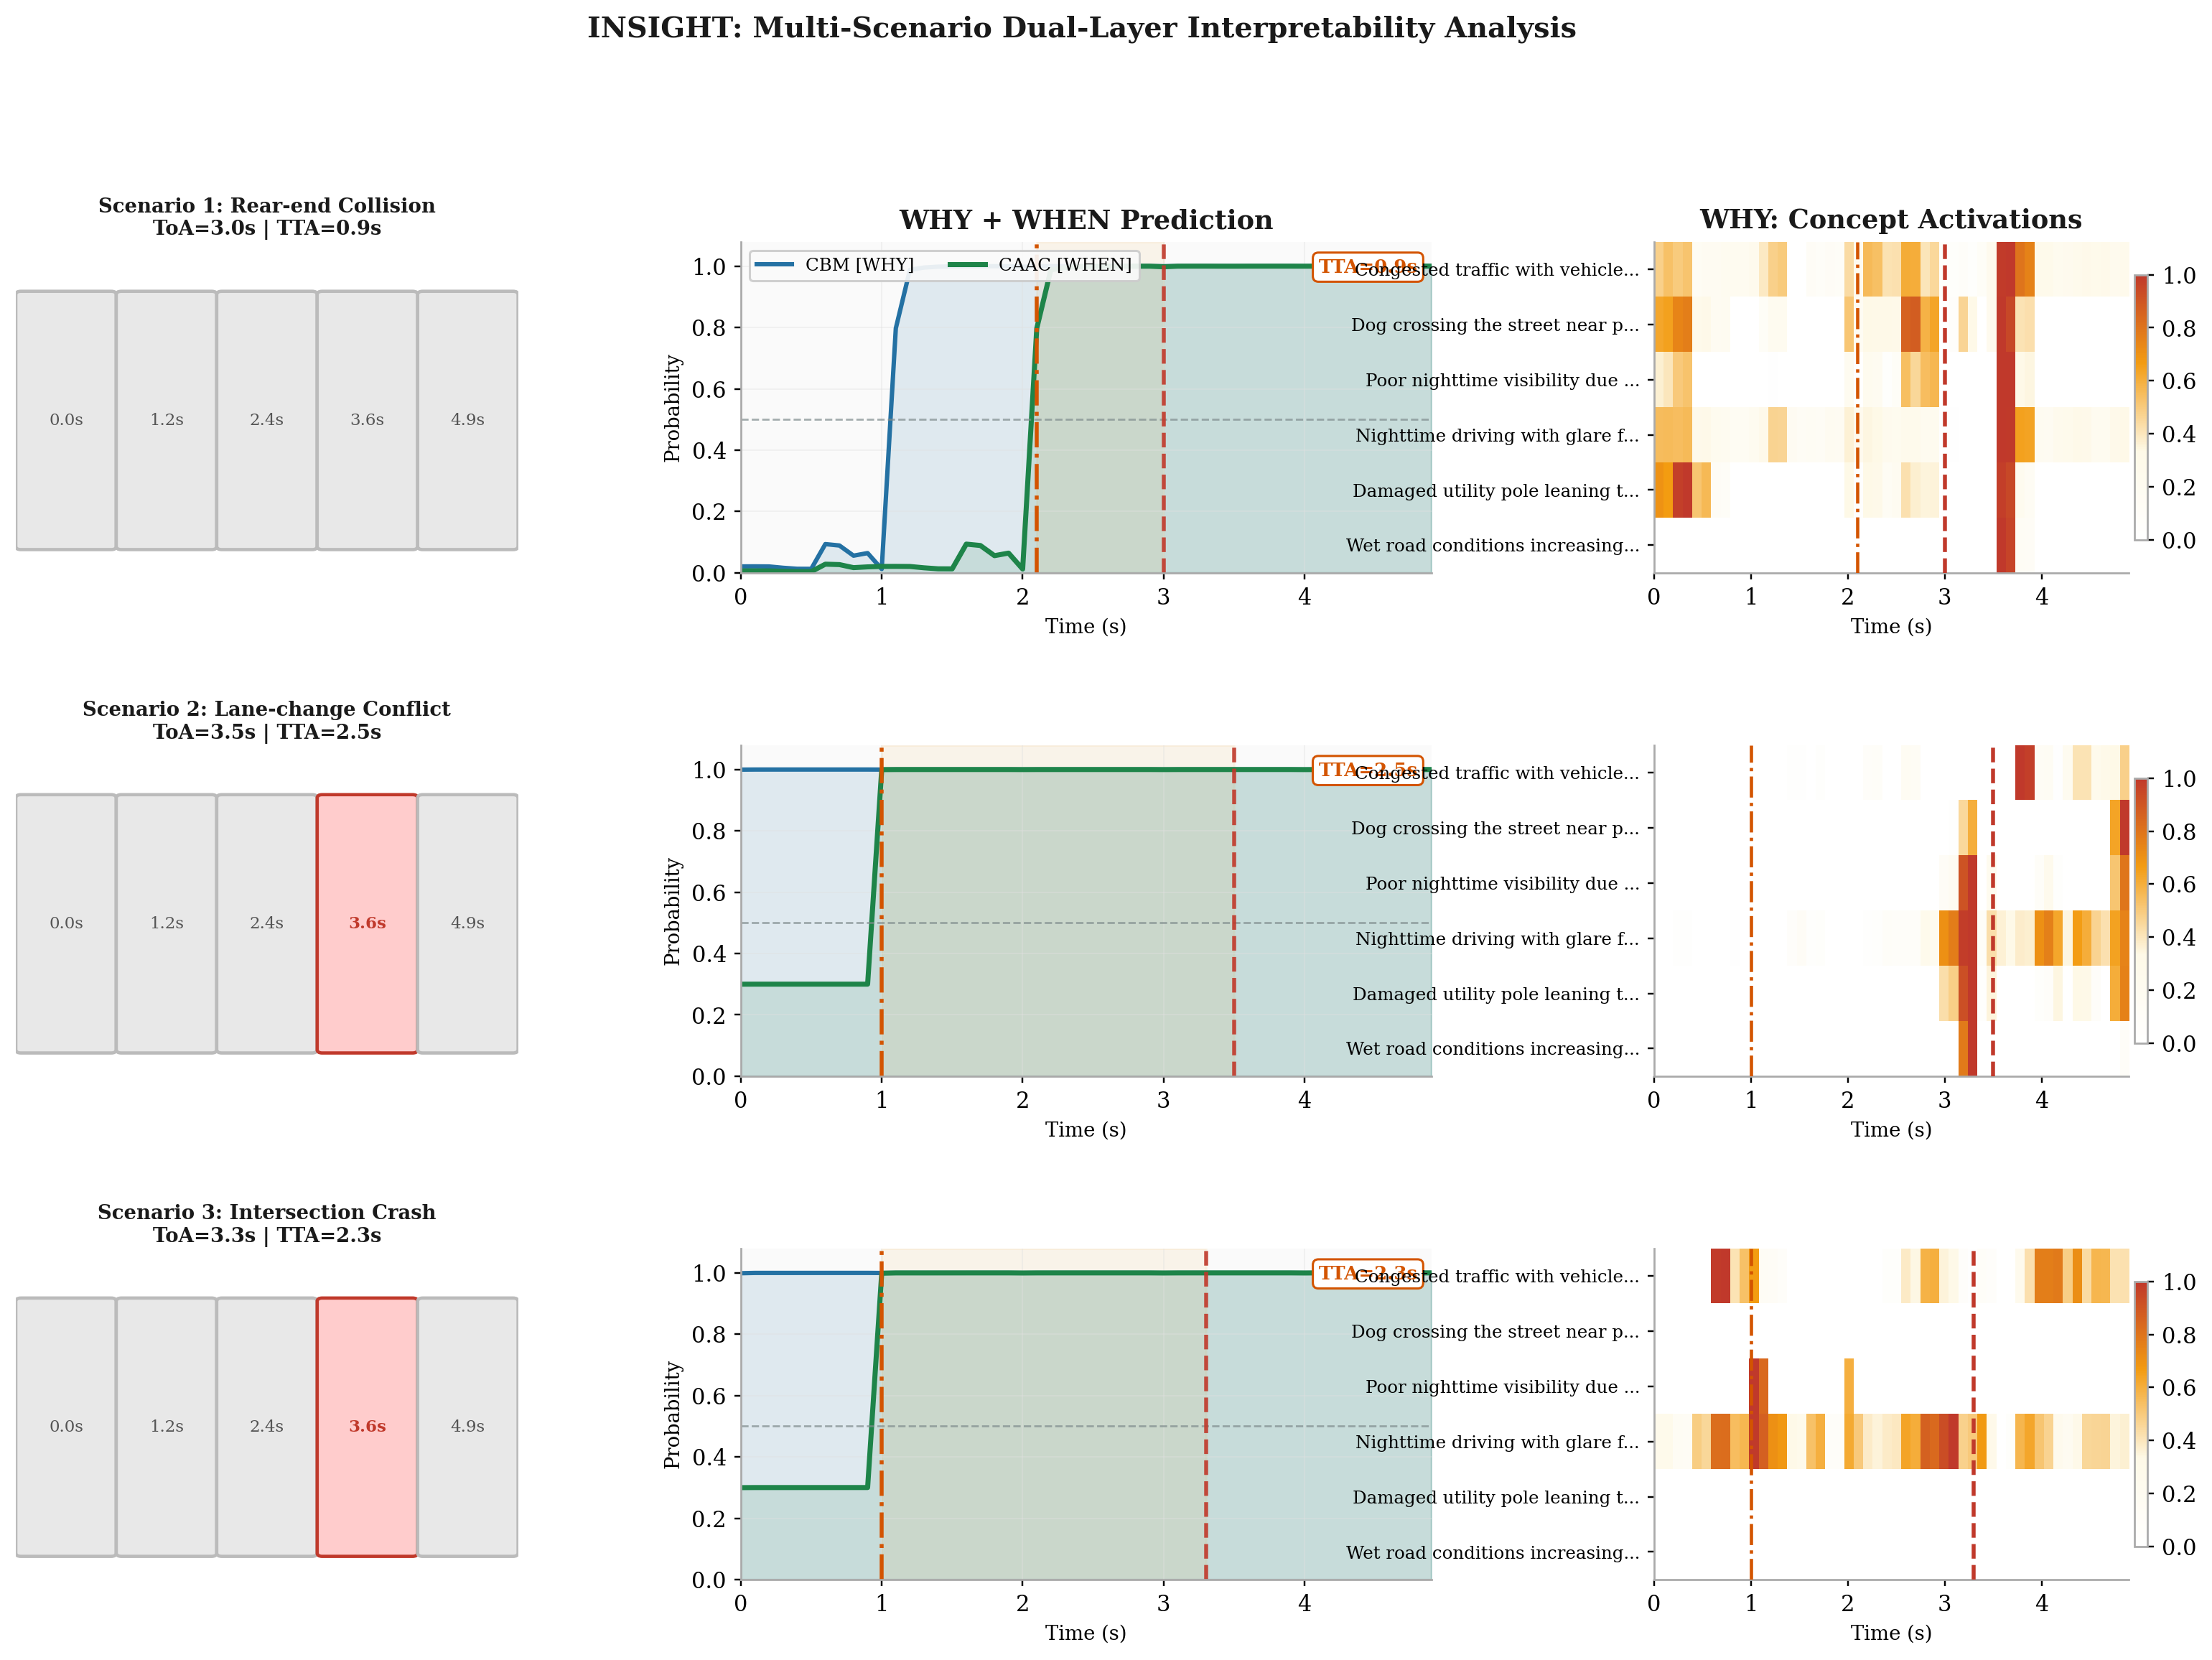
\includegraphics[width=\linewidth]{../figures/insight_fig2_multi_crash.png}
    \caption{CRASH representative trajectory}
    \label{fig:cross_dataset_bridge_traj}
  \end{subfigure}
  \hfill
  \begin{subfigure}{0.495\textwidth}
    \centering
    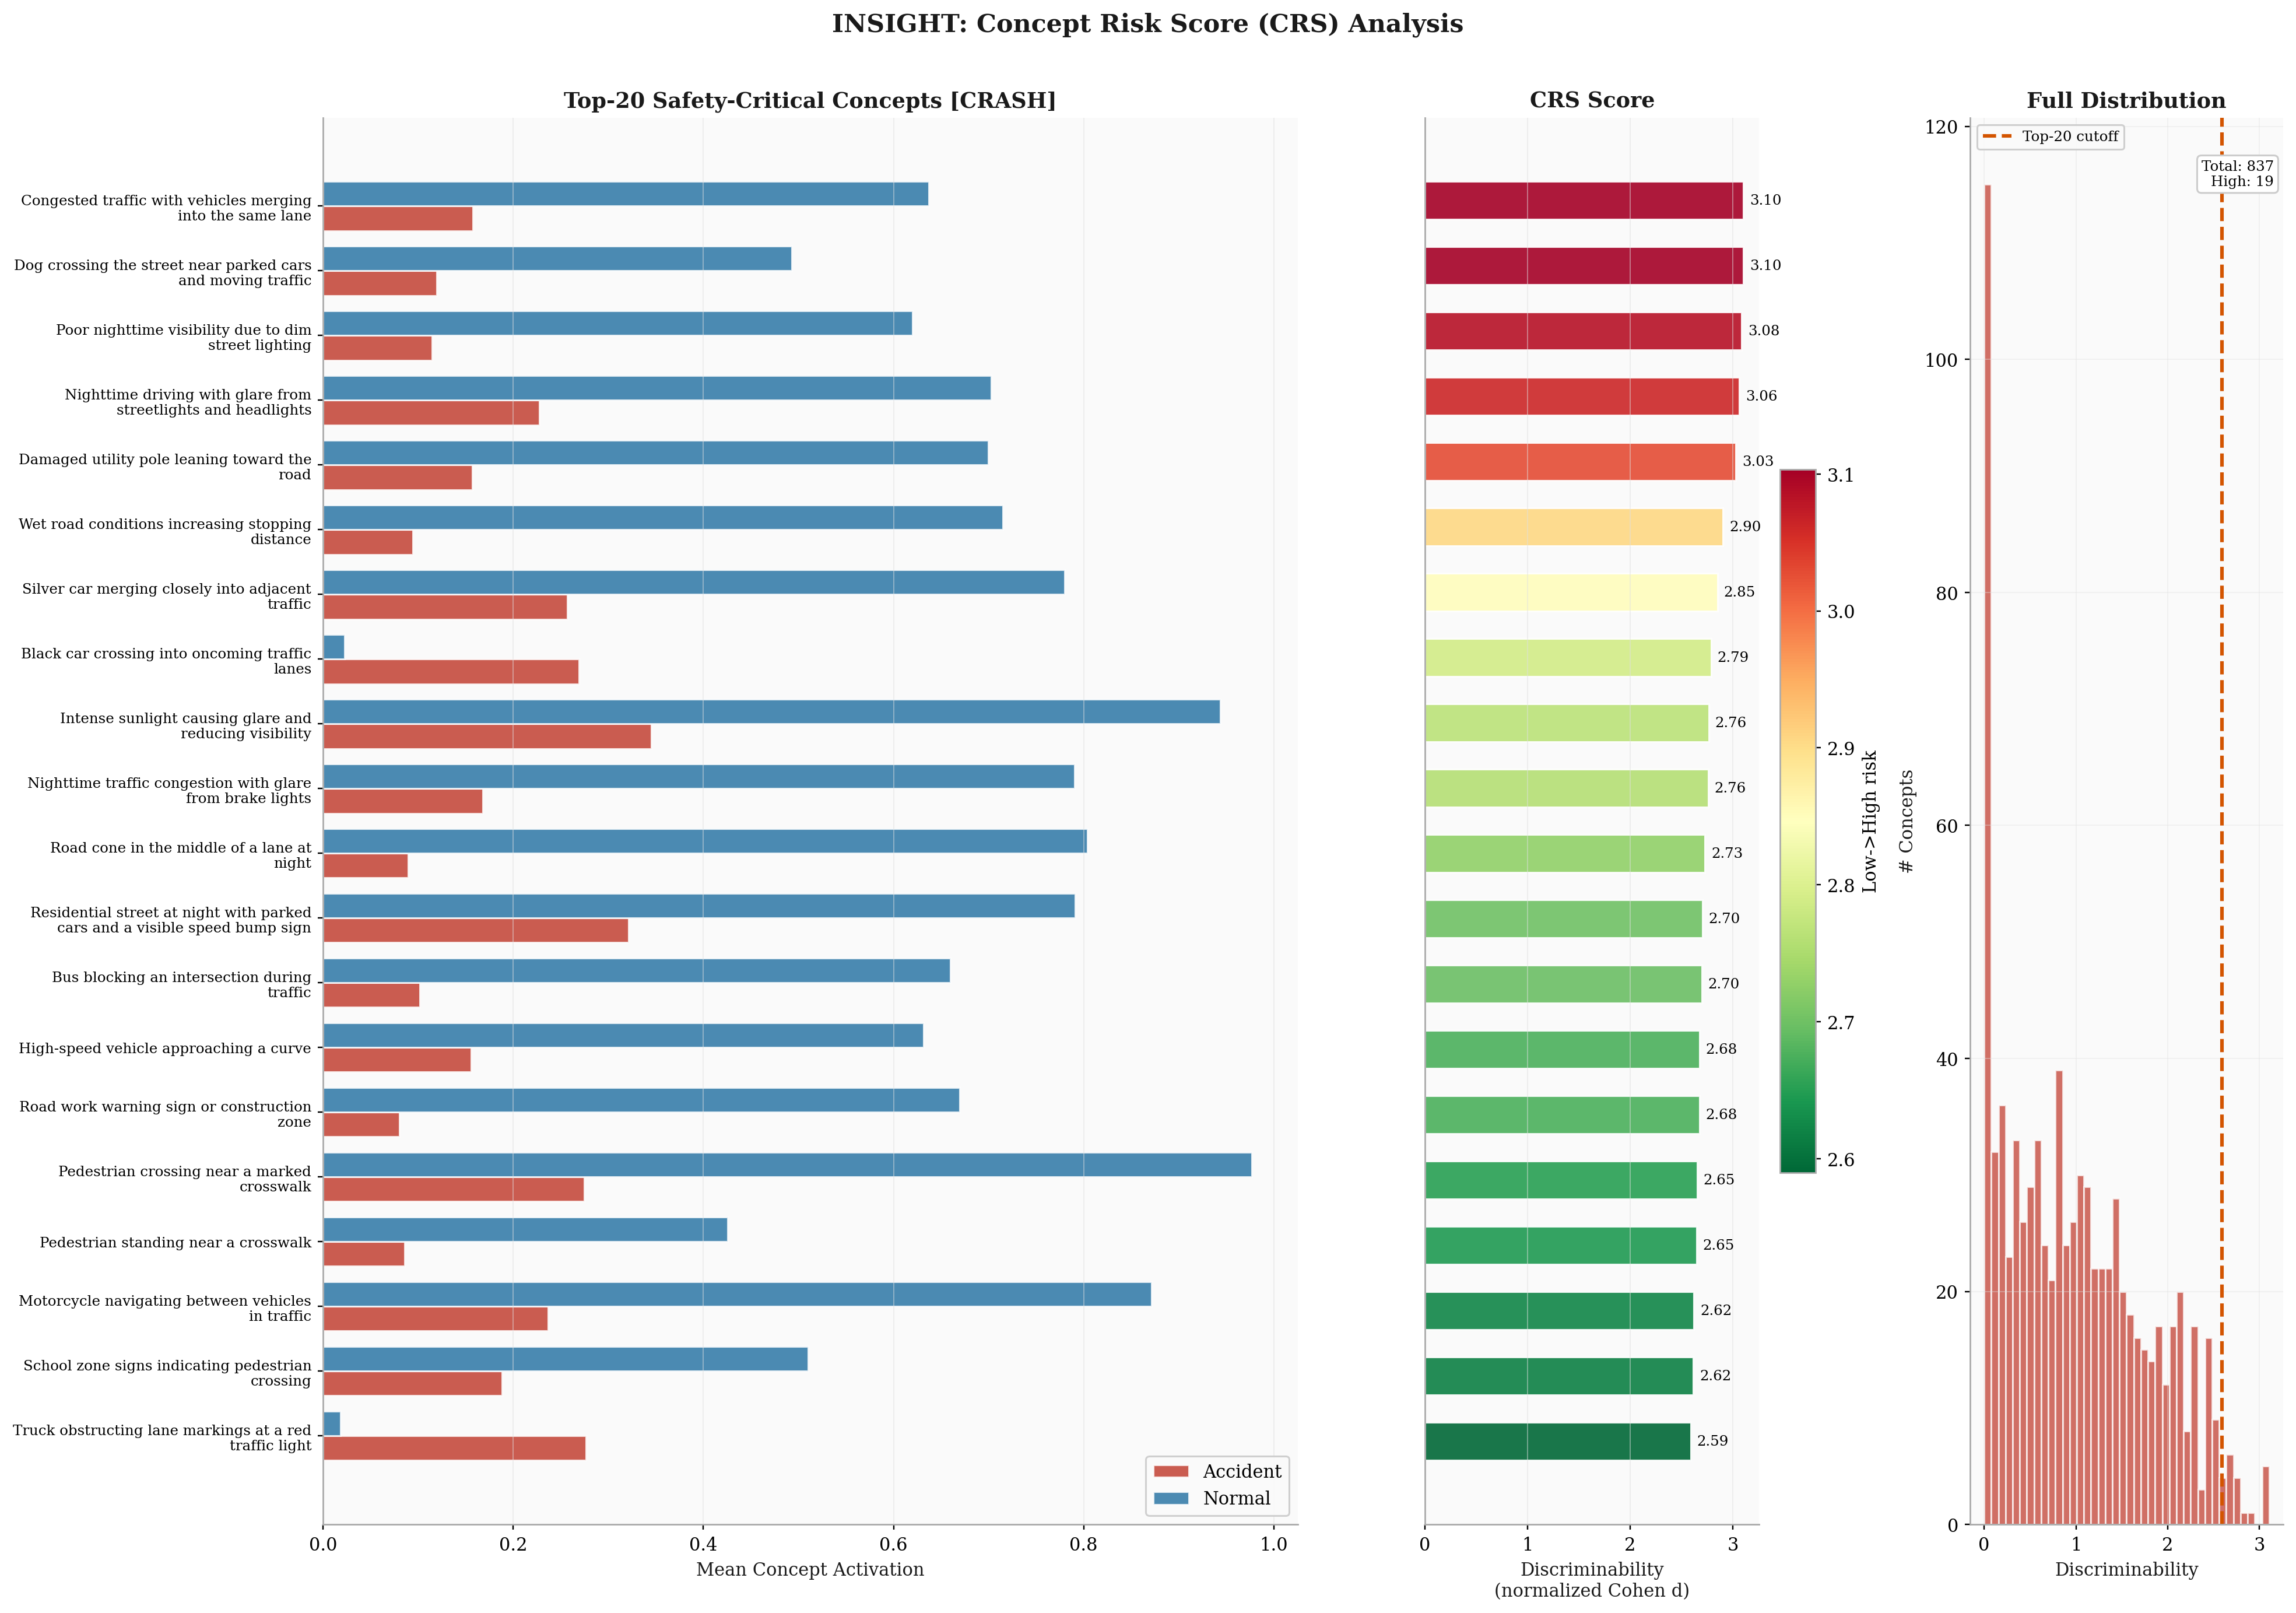
\includegraphics[width=\linewidth]{../figures/insight_fig3_crs_crash.png}
    \caption{CRASH CRS visualization}
    \label{fig:cross_dataset_bridge_crs}
  \end{subfigure}
  \caption{Cross-dataset stress bridge (support-only): CRASH cases illustrate how
  the semantic interface appears under a third corpus. These visual artifacts are
  treated as stress evidence only; headline claims remain scoped to DAD and A3D.}
  \label{fig:cross_dataset_bridge}
\end{figure*}

\paragraph{Scope and evidence envelope.}
The evaluation is deliberately designed around two datasets, not a large model
benchmark zoo. DAD and A3D are the explicit evidence corpus:
(\emph{i}) DAD serves as a noisy, short-horizon stress regime where fragility
is expected and tracked, and
(\emph{ii}) A3D serves as the cleaner regime where a semantic interface can be
interpreted as the flagship mechanism trajectory.
We do not claim dataset-agnostic dominance from this package; we claim
dataset-dependent behavioral control through a governed ontology.
\paragraph{Cross-dataset transfer note (support-only).}
To strengthen visual evidence depth, we keep one additional CRASH transfer check
as support evidence only. The archived CRASH transfer and phase-2 ablation
result files are intentionally interpreted as breadth stress signals and are not
pooled with headline DAD/A3D tables.

\subsection{Reviewer-Facing Evidence Map}
\label{sec:review-map}
\begin{figure*}[t]
\centering
\setlength{\fboxsep}{6pt}
\fbox{%
\begin{minipage}[t]{0.31\textwidth}
\textbf{Headline evidence}\\
\textbf{Use:} fast accept-level comparison\\
\textbf{Main artifacts:} Table~\ref{tab:dad}, Table~\ref{tab:a3d}, Figure~\ref{fig:safety_utility}\\
\textbf{Reading:} A3D is the clean flagship operating point; DAD headline is reported but not overstated.
\end{minipage}}
\hfill
\fbox{%
\begin{minipage}[t]{0.31\textwidth}
\textbf{Controlled support evidence}\\
\textbf{Use:} test ontology/mechanism under matched launchers\\
\textbf{Main artifacts:} Table~\ref{tab:concept_sets}, Table~\ref{tab:ablation}, Figure~\ref{fig:qual_case_stress}\\
\textbf{Reading:} ontology choice is an empirical variable; support blocks are not pooled as leaderboard claims.
\end{minipage}}
\hfill
\fbox{%
\begin{minipage}[t]{0.31\textwidth}
\textbf{Stress evidence}\\
\textbf{Use:} boundary and failure-mode disclosure\\
\textbf{Main artifacts:} DAD robustness paragraphs, Table~\ref{tab:interp_quant}, appendix intervention logs\\
\textbf{Reading:} DAD remains fragile stress evidence; actor-policy timing remains scoped support.
\end{minipage}}
\caption{[Reading-map evidence] Visual evidence map for rapid claim-tier reading. The paper separates
headline, controlled support, and stress evidence so each claim has one role
and one interpretation tier.}
\label{fig:review_map}
\end{figure*}

\paragraph{Pseudo-label sensitivity.}
We also audited the top-$m$ CLIP pseudo-label recipe on a larger 500-frame DAD
slice from the paper ontology. The main takeaway remains pragmatic: top-3 is a
reasonable middle ground. In this audit, top-1 activates only one semantic
family per frame on average and captures 5.5\% of the cumulative top-20
similarity mass, while top-10 spreads across 5.14 families and absorbs 51.5\%
of that mass. Top-3 sits between these extremes with 2.34 families per frame
and 16.0\% relative mass, so we retain it in the main recipe as a practical
balance between coverage and noise rather than as a claim of exact semantic
calibration.

\paragraph{Verbalization robustness.}
We also measured whether canonical paper-facing concept names remain stable
under light paraphrase changes. Across 12 canonical concepts with two variants
each, canonical and variant prompts achieve mean text cosine 0.939, mean
frame-score correlation 0.887, mean top-10 frame overlap 0.525, and mean
absolute score difference 0.013 on the same 500-frame DAD audit. These results
support the paper's naming policy: short canonical risk phrases remain stable
anchors for the semantic interface, even though a few more abstract paraphrases
are visibly weaker.

Taken together, the pseudo-label and paraphrase audits address two different
language-side failure modes. The top-$m$ audit checks whether the semantic
bootstrap is too concentrated or too diffuse, while the paraphrase audit checks
whether the paper-facing ontology is brittle to minor wording changes. Together
with the family-balance and merge-provenance assets in the appendix, these
analyses justify treating the ontology as a governed language interface rather
than as a hidden prompt artifact.

\subsection{Interpretability Taxonomy of Prior Work}

\begin{table}[t]
\caption{[Controlled support evidence] Interpretability taxonomy for accident anticipation. The point of this
table is not that every method should expose the same type of explanation, but
that most prior systems still lack an explicit semantic interface that can be
trained, audited, and compared across runs.}
\label{tab:interp_comparison}
\centering\small
\setlength{\tabcolsep}{4pt}
\resizebox{\linewidth}{!}{%
\begin{tabular}{lcccc}
\toprule
Method & Semantic state & Timing account & Intrinsic? & Params\\
\midrule
DSA-RNN~\citep{ref4}         & \texttimes & \texttimes & -- & 12M\\
DRIVE~\citep{ref2}           & Grad-CAM & RL-trained attention & post-hoc & 31M\\
DSTA~\citep{ref17}           & \texttimes & \texttimes & -- & 180M\\
DAA-GNN~\citep{ref32}        & \texttimes & \texttimes & -- & 183M\\
W3AL~\citep{liao2024and}     & verbal localisation & verbal timing & post-hoc & 7B\\
CRASH~\citep{liao2024crash}  & \texttimes & \texttimes & -- & 26M\\
CCAF-Net~\citep{liu2025ccaf} & \texttimes & \texttimes & -- & 191M\\
LATTE~\citep{ZHANG2025103173}& \texttimes & \texttimes & -- & 45M\\
\midrule
\textbf{\method{} (Ours)} & \textbf{concept bottleneck} &
\textbf{concept-conditioned timing} & \textbf{\checkmark} & \textbf{30M}\\
\bottomrule
\end{tabular}%
}
\end{table}

Table~\ref{tab:interp_comparison} highlights the representational gap that
motivates our paper. Prior methods may be highly predictive, but most do not
provide a trainable semantic layer that links named risk concepts to downstream
anticipation behavior. \method{} closes that gap architecturally. Empirically,
the paper is strongest on the semantic layer and on ontology-controlled
comparisons, with timing analyses reported as a downstream extension of the
same interface.

\subsection{Main Predictive Results on DAD}

\begin{table}[t]
\caption{[Headline evidence] DAD results. We separate interpretable or
explanation-oriented methods
from strong non-interpretable references to position \method{} as a competitive
interpretable system with an explicit semantic interface.}
\label{tab:dad}
\centering\small
\setlength{\tabcolsep}{4pt}
\resizebox{\linewidth}{!}{%
\begin{tabular}{lcccc}
\toprule
Method & Venue & AP$\uparrow$ & mTTA$\uparrow$ & Interface\\
\midrule
DSA-RNN~\citep{ref4}        & ACCV'16 & 38.1\% & 2.05s & none\\
DRIVE~\citep{ref2}          & ICCV'21 & 58.4\% & 2.31s & post-hoc\\
DSTA~\citep{ref17}          & TITS'22 & 56.1\% & 3.66s & none\\
Graph$^2$~\citep{ref36}     & WACV'24 & 64.8\% & 2.98s & none\\
DAA-GNN~\citep{ref32}       & PR'24 & 75.2\% & 1.59s & none\\
W3AL~\citep{liao2024and}    & MM'24 & 69.2\% & -- & verbal\\
CRASH~\citep{liao2024crash} & MM'24 & 65.3\% & 1.75s & none\\
\midrule
\method{} (Ours) & -- & 68.19\% & 1.75s & semantic\\
\midrule
$\dagger$ CCAF-Net & -- & 81.3\% & 4.15s & none\\
$\dagger$ LATTE & -- & 89.7\% & 4.49s & none\\
\bottomrule
\end{tabular}%
}
\end{table}

\method{} reaches 68.19\% AP and 1.75s mTTA on the canonical DAD curriculum
line. This result shows that an explicit semantic interface can remain
competitive on DAD while providing a more auditable representation than prior
interpretable or explanation-oriented baselines. We report it as the endpoint
of the canonical curriculum line, with separate multi-seed diagnostics below to
make the DAD stability profile explicit.

\paragraph{Multi-seed robustness (DAD, curriculum line).}
To quantify checkpoint sensitivity, we launched three clean seeds under the
same curriculum family and reported synchronized epochs rather than per-seed
best test checkpoints. At epoch~25, the three-seed aggregate is
$\text{AP}=56.39\%\pm3.46$ and $\text{mTTA}=2.40\pm0.05$~s.
At epoch~30, the aggregate is $\text{AP}=55.16\%\pm3.63$ and
$\text{mTTA}=2.49\pm0.09$~s. We include these numbers as a checkpoint-sensitivity
diagnostic, not as a replacement for the canonical headline line. Their role
is to show that DAD remains more fragile than A3D and that the paper is
explicit about that fragility.

As a follow-up stress envelope, we also completed the fixed-vocabulary
\texttt{dad\_curriculum\_v2} recovery family. The clean three-seed set is
$62.31\%\pm1.90$ AP with $2.07\pm0.09$~s mTTA; the recovery three-seed set is
$63.64\%\pm0.80$ AP with $2.33\pm0.27$~s mTTA. Combining clean plus recovery
snapshots yields $63.72\%\pm2.35$ AP and $2.14\pm0.27$~s mTTA. These values
reinforce that DAD performance is measurable under stress but that the frontier
is noisier than in A3D. Detailed per-run logs are kept in the curriculum-recovery
support status file.

\paragraph{DAD mechanism-hardening block (support-only).}
A predeclared support block targeting DAD mechanism fragility has completed with
3/3 clean seeds. Under matched settings, the completed aggregate is
$63.18\%\pm1.32$ AP and $2.27\pm0.20$~s mTTA (sampled at synchronized
support checkpoints).
This block narrows but does not overturn the broader interpretation:
DAD remains a high-variance stress test for this method family, while the
semantic-interface framing stays stable.

\paragraph{Low-regularization follow-up (support-only).}
The low-regularization mechanism-hardening follow-up has also completed at 3/3.
Its aggregate is $64.42\%\pm0.97$ AP and $2.35\pm0.20$~s mTTA.
By the internal interpretation gate, this is a useful-tie stress outcome and does
not promote DAD to the headline mechanism claim.
\begin{figure*}[t]
\centering
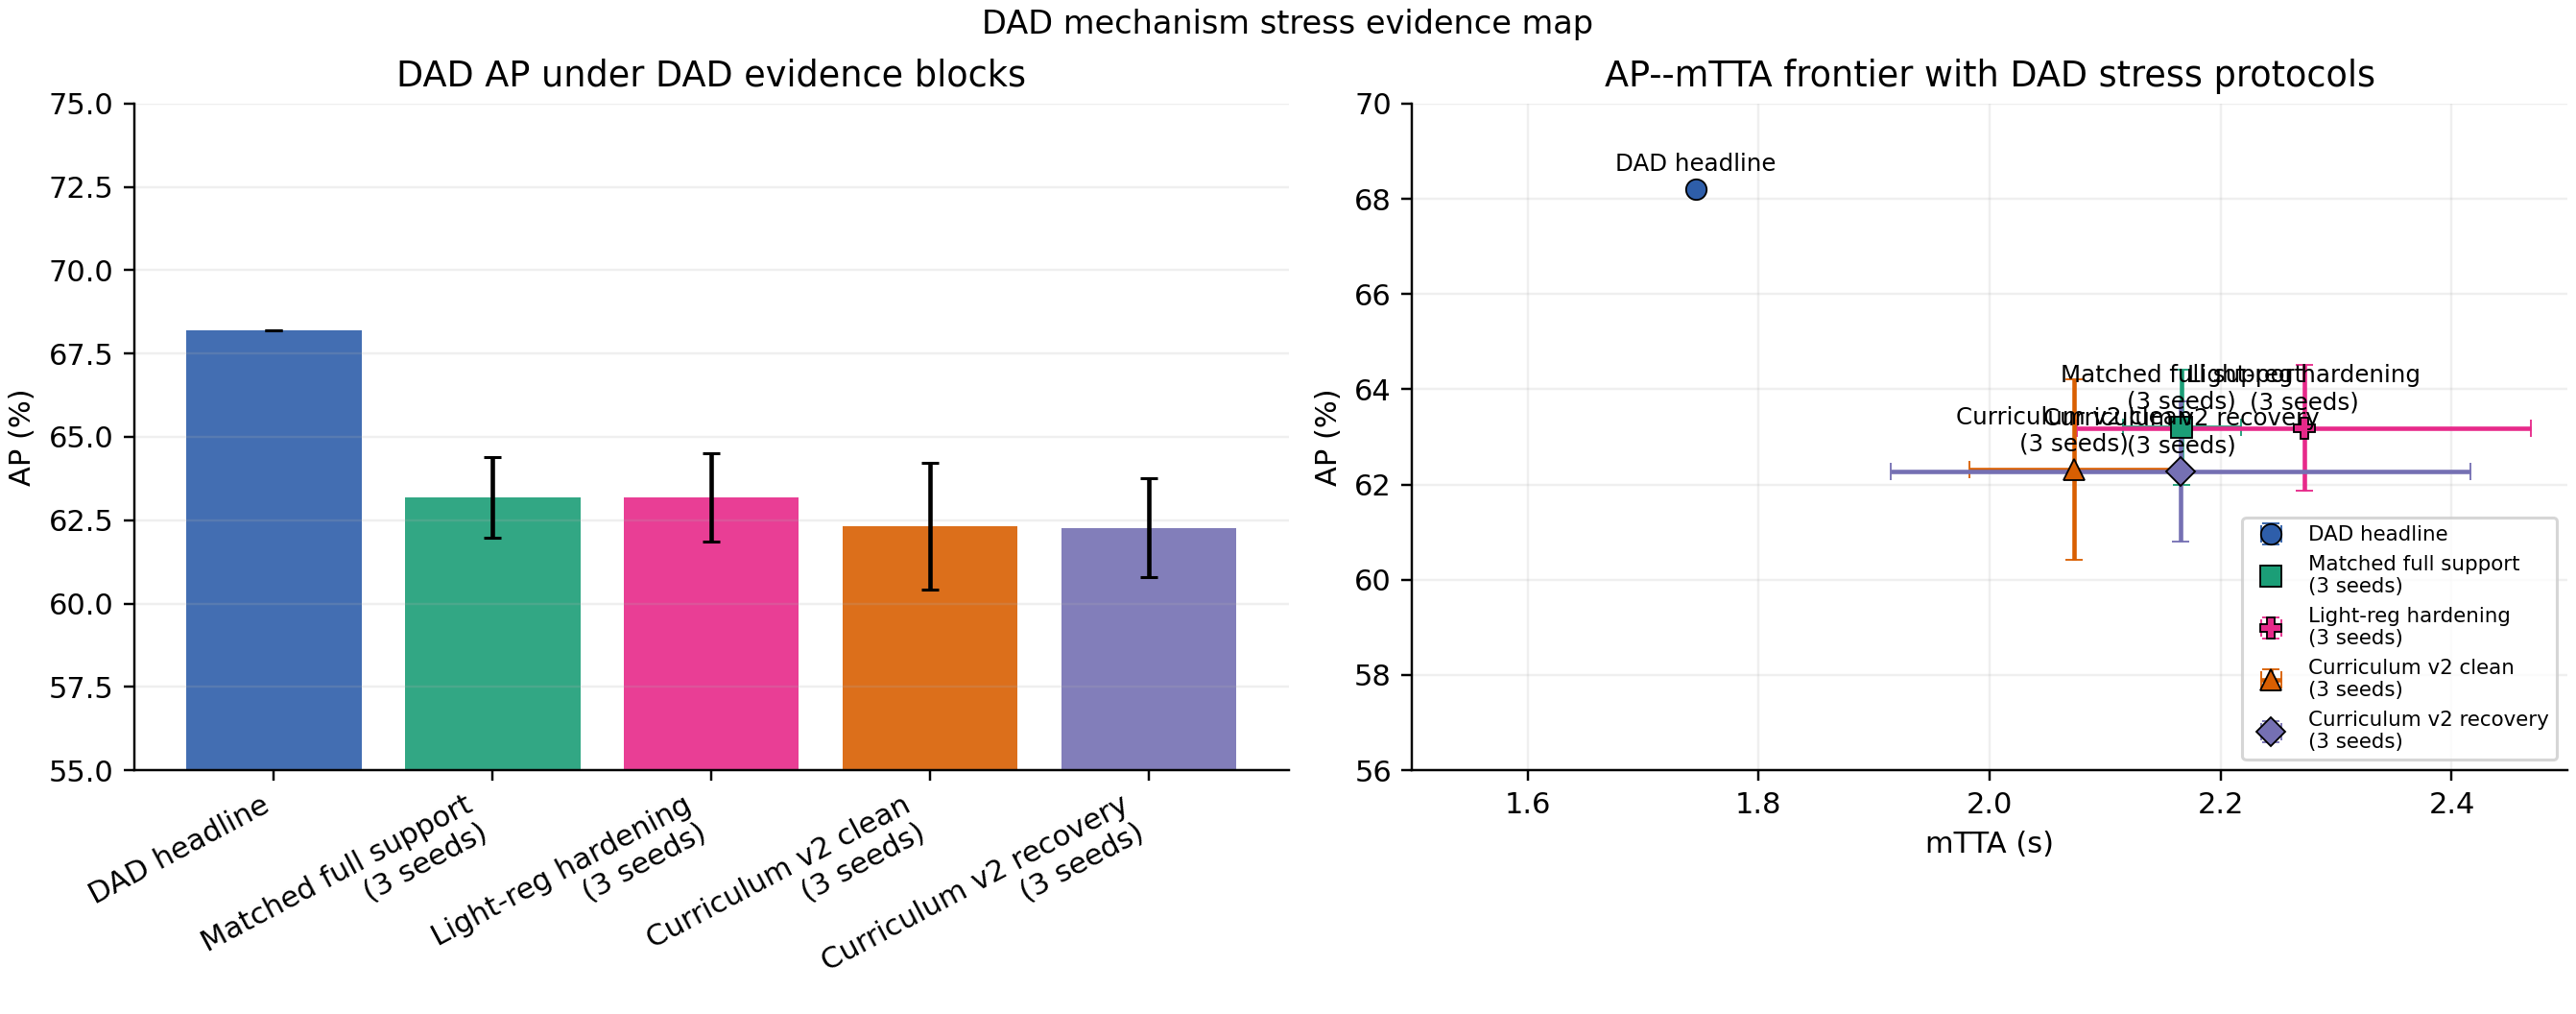
\includegraphics[width=0.98\textwidth]{../figures/insight_fig6_dad_stress_summary.pdf}
\caption{[Mechanism stress evidence] DAD mechanism-stress evidence across protocol blocks. We report three
support tiers against the canonical headline run: matched full-support,
light-regularization hardening, and curriculum-recovery expansion. Error bars
mark seed-level mean and standard deviation on AP and mTTA so the stress-story is
read as a frontier band rather than a single favorable point.}
\label{fig:dad_stress_summary}
\end{figure*}

\subsection{Main Predictive Results on A3D}

\begin{table}[t]
\caption{[Headline evidence] A3D results. \method{} reaches a strong
interpretable operating point
with better warning lead time than CRASH while maintaining competitive AP.}
\label{tab:a3d}
\centering\small
\setlength{\tabcolsep}{3pt}
\resizebox{\linewidth}{!}{%
\begin{tabular}{lccccc}
\toprule
Method & AP$\uparrow$ & mTTA$\uparrow$ & TTA@R80$\uparrow$ & P@R80$\uparrow$ & Interface\\
\midrule
CRASH~\citep{liao2024crash} & 96.0\% & 4.27s & -- & -- & none\\
W3AL~\citep{liao2024and}    & 92.4\% & 4.52s & -- & -- & verbal\\
\midrule
\method{} & 93.4\% & 4.90s & 4.89s & 0.9067 & semantic\\
$\Delta$ vs.\ CRASH & $-2.60\%$ & $+14.8\%$ & -- & -- & --\\
\bottomrule
\end{tabular}%
}
\end{table}

On A3D, \method{} achieves a stronger and cleaner paper-facing result. The
model improves mTTA over CRASH while maintaining competitive AP, which places
it in a favorable interpretable region of the accuracy--timeliness plane.
Because A3D offers more progressive hazard development than DAD, it also serves
as the dataset where the semantic-interface story is easiest to read:
conceptual precursors appear early enough to support both prediction and
auditing.

\paragraph{A3D headline stability.}
The flagship A3D recipe also remains stable across three seeds. A dedicated
headline audit yields $\text{AP}=94.16\%\pm0.95$ and
$\text{mTTA}=4.62\pm0.42$~s, which matters because A3D is the paper's cleanest
semantic-interface dataset. This multi-seed result does not change the main
claim, but it makes the strongest table in the paper materially more stable
under scrutiny.

\begin{figure*}[t]
\centering
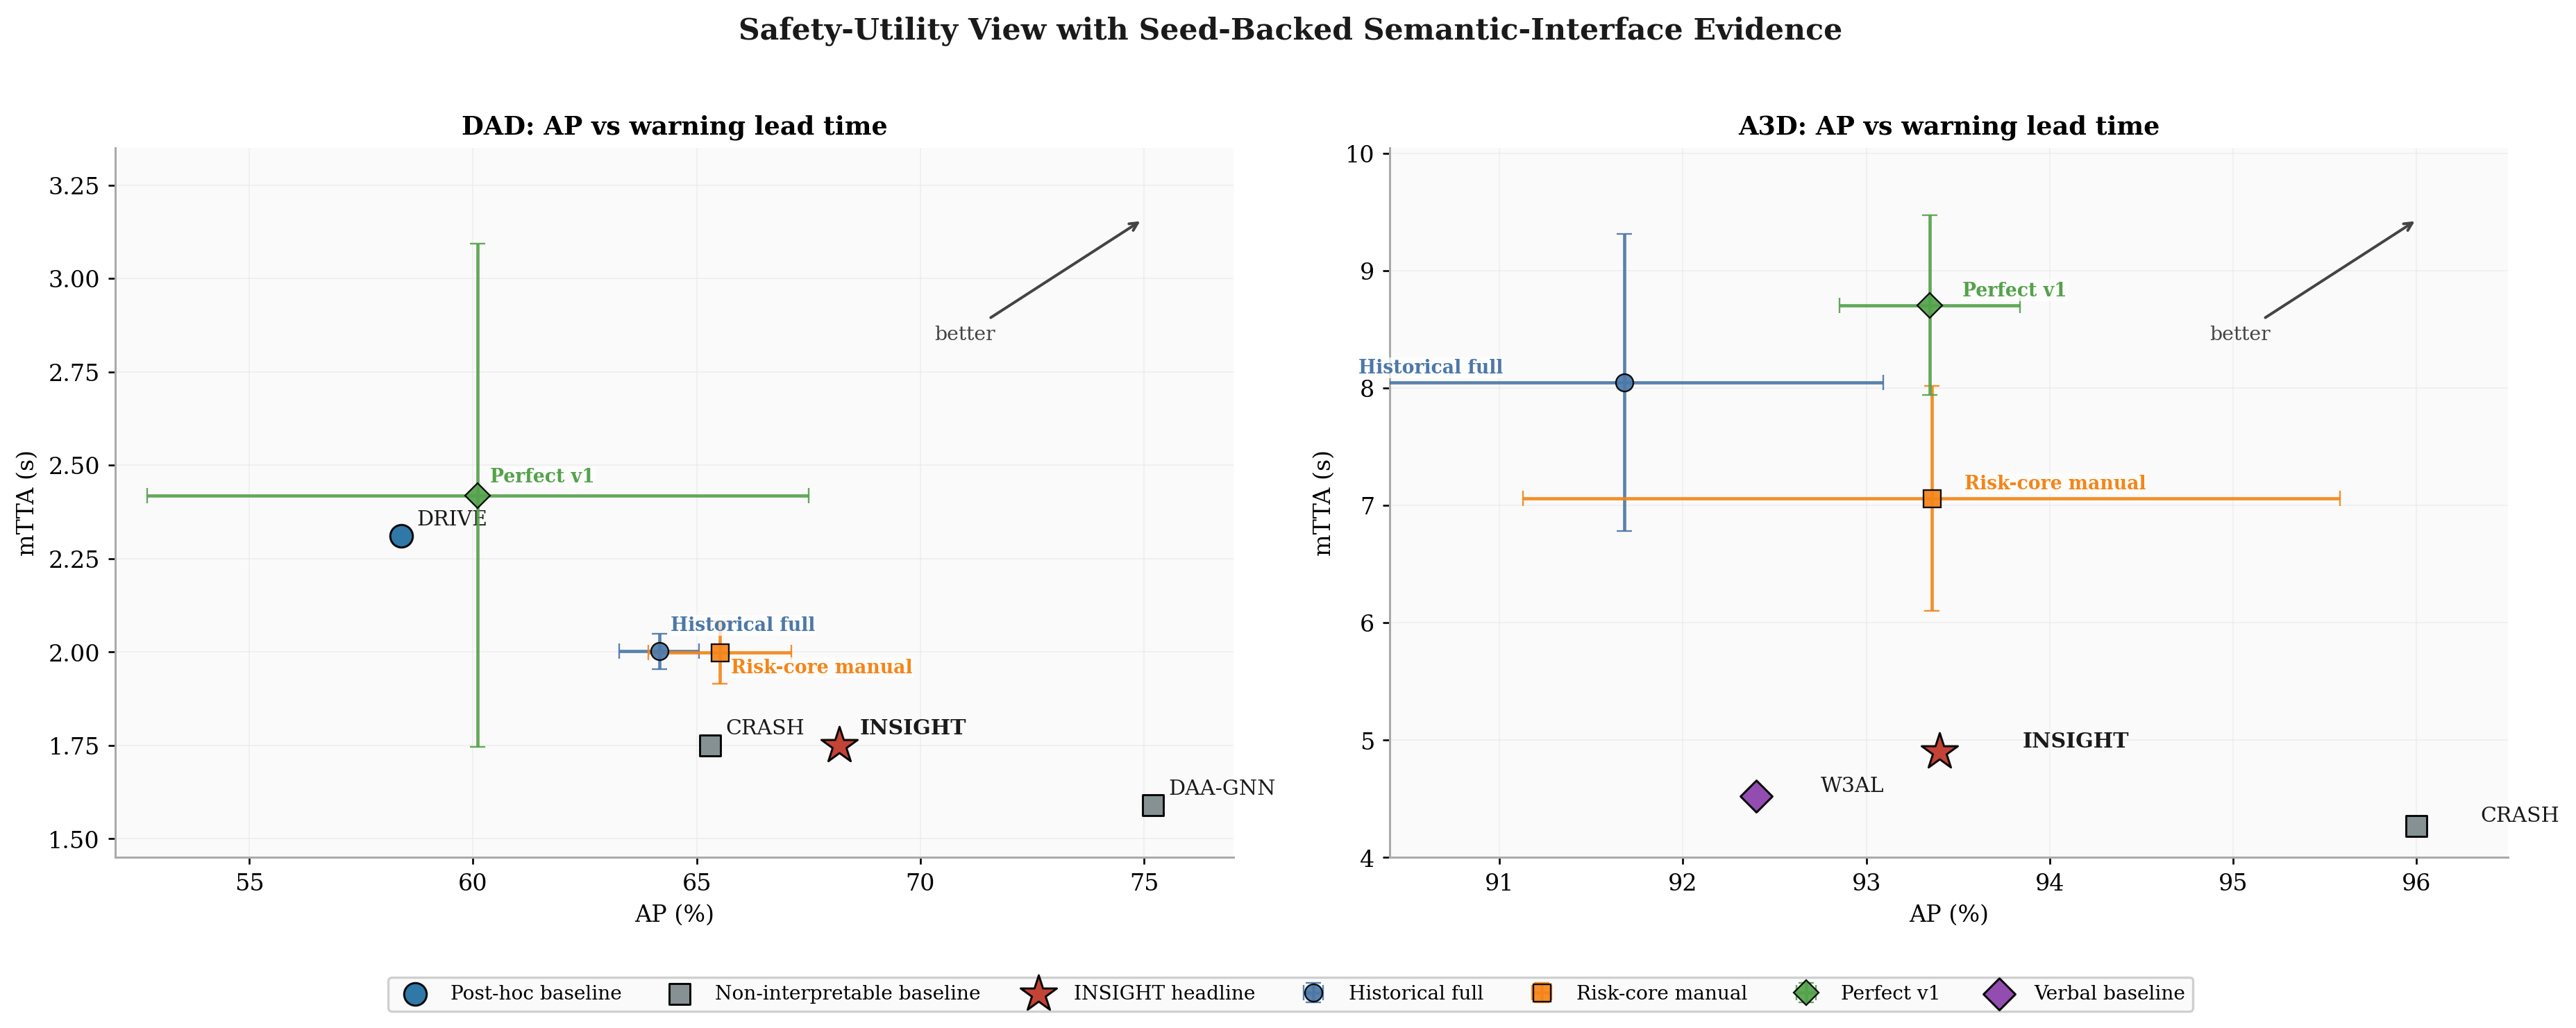
\includegraphics[width=0.98\textwidth]{../figures/insight_fig5_safety_utility.pdf}
\caption{[Reading bridge: headline + controlled support] Safety--utility view under semantic-interface constraints. Literature
baselines and headline \method{} points are shown as table values, while the
colored ontology markers show three-seed matched-launcher aggregates with
horizontal AP and vertical mTTA standard-deviation intervals. The figure makes
the evidence tiers explicit: \method{} occupies a competitive interpretable
operating point, and ontology choice measurably moves the AP--mTTA frontier.}
\label{fig:safety_utility}
\end{figure*}

Figure~\ref{fig:safety_utility} complements the tables by making the paper's
position explicit: the target operating regime is strong anticipation with an
auditable semantic layer.

\subsection{Ontology Choice Changes the Operating Point}

\begin{table*}[t]
\caption{[Controlled support evidence] Matched ontology comparison under the
shared launcher protocol. Only
the ontology source varies; the training launcher family is held fixed.}
\label{tab:concept_sets}
\centering\small
\begin{tabular}{llccccc}
\toprule
Dataset & Concept set & \#Concepts & AP$\uparrow$ & mTTA$\uparrow$ & TTA@R80$\uparrow$ & P@R80$\uparrow$\\
\midrule
DAD & Historical full & 837 & 64.91\% & 1.88s & 2.51s & 0.492 \\
DAD & Risk-core manual & 30 & \textbf{65.25\%} & 2.15s & \textbf{2.92s} & 0.462 \\
DAD & Perfect concept set v1 & 80 & 64.15\% & \textbf{2.30s} & 2.67s & 0.467 \\
\midrule
A3D & Historical full & 837 & 93.88\% & 9.41s & 8.13s & 0.940 \\
A3D & Risk-core manual & 30 & 94.36\% & \textbf{9.57s} & \textbf{8.60s} & \textbf{0.944} \\
A3D & Perfect concept set v1 & 80 & \textbf{96.54\%} & 8.69s & 7.11s & 0.934 \\
\bottomrule
\end{tabular}
\end{table*}

Table~\ref{tab:concept_sets} is one of the most important result blocks in the
paper. It shows that ontology choice changes the AP--mTTA frontier rather than
yielding one universally dominant vocabulary. On DAD, the compact manual set
has the highest AP under the shared recipe, while the polished discovered
ontology gives the best mTTA. On A3D, the discovered ontology achieves the
strongest AP, while the compact manual set gives the best timing metrics. The
scientific lesson is that ontology design is not decoration: it is an
experimental variable that changes downstream behavior. This is the paper's
most direct evidence that language-side design decisions survive contact with
model training: changing canonical names, merge policy, and family structure at
the ontology level changes the downstream operating point under one matched
launcher family.

This claim is now backed by a complete three-seed extension over all six
dataset--ontology cells. Across the matched ontology block, all $18/18$
recommended seeded runs are finished. On A3D, the paper-facing discovered
ontology remains competitive under this aggregate view
($93.35\%\pm0.49$ AP, $8.71\pm0.77$~s mTTA), so the ontology effect is not
resting on one favorable seed. On DAD, however, the discovered ontology shows
substantially larger variance ($60.11\%\pm7.40$ AP), which is exactly why we
continue to describe DAD as the fragile side of the paper rather than trying
to oversell a uniform robustness story.

\subsection{Current Timing and Intervention Evidence}

\begin{table}[t]
\caption{[Mechanism stress evidence] Matched score-source comparison on
representative checkpoints. The
same trained checkpoint is evaluated twice: once with the classifier score
trajectory and once with the actor policy score trajectory. These are support
analyses, not canonical headline results.}
\label{tab:trigger_compare}
\centering\small
\setlength{\tabcolsep}{3pt}
\resizebox{\linewidth}{!}{%
\begin{tabular}{llcccc}
\toprule
Dataset & Score source & AP$\uparrow$ & mTTA$\uparrow$ & TTA@R80$\uparrow$ & P@R80$\uparrow$\\
\midrule
DAD & classifier & 61.94\% & 2.16s & 2.87s & 0.486 \\
DAD & actor & 34.67\% & 2.08s & 5.00s & 0.349 \\
\midrule
A3D & classifier & 93.88\% & 4.71s & 4.06s & 0.940 \\
A3D & actor & 91.14\% & 4.97s & 4.94s & 0.911 \\
\bottomrule
\end{tabular}%
}
\end{table}

Table~\ref{tab:trigger_compare} clarifies the scope of the timing claim. On
A3D, actor-based evaluation is fairly close to the classifier line on a
representative checkpoint, suggesting that concept-conditioned timing is
plausible beyond the classifier trajectory. On DAD, actor-based evaluation is
still substantially weaker, which is why the paper continues to report
classifier-derived headline metrics. This is precisely why we do not let the
actor branch carry the main paper claim. This comparison therefore works best
as a transfer test: it shows how much timing behavior survives when we switch
from the classifier trajectory to the learned actor policy.

An extended DAD trigger-source audit over six same-family support checkpoints
reinforces this cautious reading rather than weakening it. Across that block,
classifier-based evaluation averages $61.11\%\pm4.58$ AP and
$2.17\pm0.19$~s mTTA, whereas actor-based evaluation averages
$37.41\%\pm7.35$ AP and $3.73\pm1.39$~s mTTA. The actor's threshold-crossing
rate is also unstable across checkpoints, which means the current policy
branch should still be read as partial timing evidence rather than as a mature
replacement for classifier-derived anticipation scores.

Archived prediction-timing analyses nevertheless provide useful support for the
semantic interface story. The classifier branch crosses threshold before impact
on many positive cases, and archived concept amplification experiments show that
positive concept edits can move alerts earlier on a non-trivial subset of
valid edited cases. Together, these results show that the interface is
structurally meaningful and partially intervenable, while a complete
policy-level causal timing account lies beyond the current paper.

\subsection{Ontology Quality as Evidence, Not Decoration}

The ontology work is not merely qualitative preprocessing. The paper-facing
artifacts record a source pool of more than 600 candidate phrases, an
order-of-magnitude compression to a paper-ready ontology of about 80 concepts,
family-balance audits across nine semantic families, canonical merge examples,
and light human review notes. The point of these assets is scientific
accountability: if ontology construction is part of the method, then the
ontology itself should be inspectable, comparable, and citable as evidence.
This is one of the main differences between our approach and systems that
inherit their semantic vocabularies implicitly. For EMNLP, this evidence block
is central: the contribution is not only that the model has concepts, but that
the exposed semantic layer is named, canonicalized, reviewable, and tied to
explicit provenance.

Concretely, the paper-facing audit trail compresses 611 mined phrases into a
post-polish pool of 81 canonical candidates and a finalized release of 80
reviewed concepts. The retained vocabulary is distributed across nine explicit
families, and the current human-review log covers all 80 retained concepts with
light-touch keep decisions rather than ontology rebuilding. We view this as an
important distinction: the paper is not claiming a finished lexical resource,
but a governed semantic interface whose canonical names, family coverage, and
merge provenance can be inspected directly.

\begin{figure}[t]
\centering
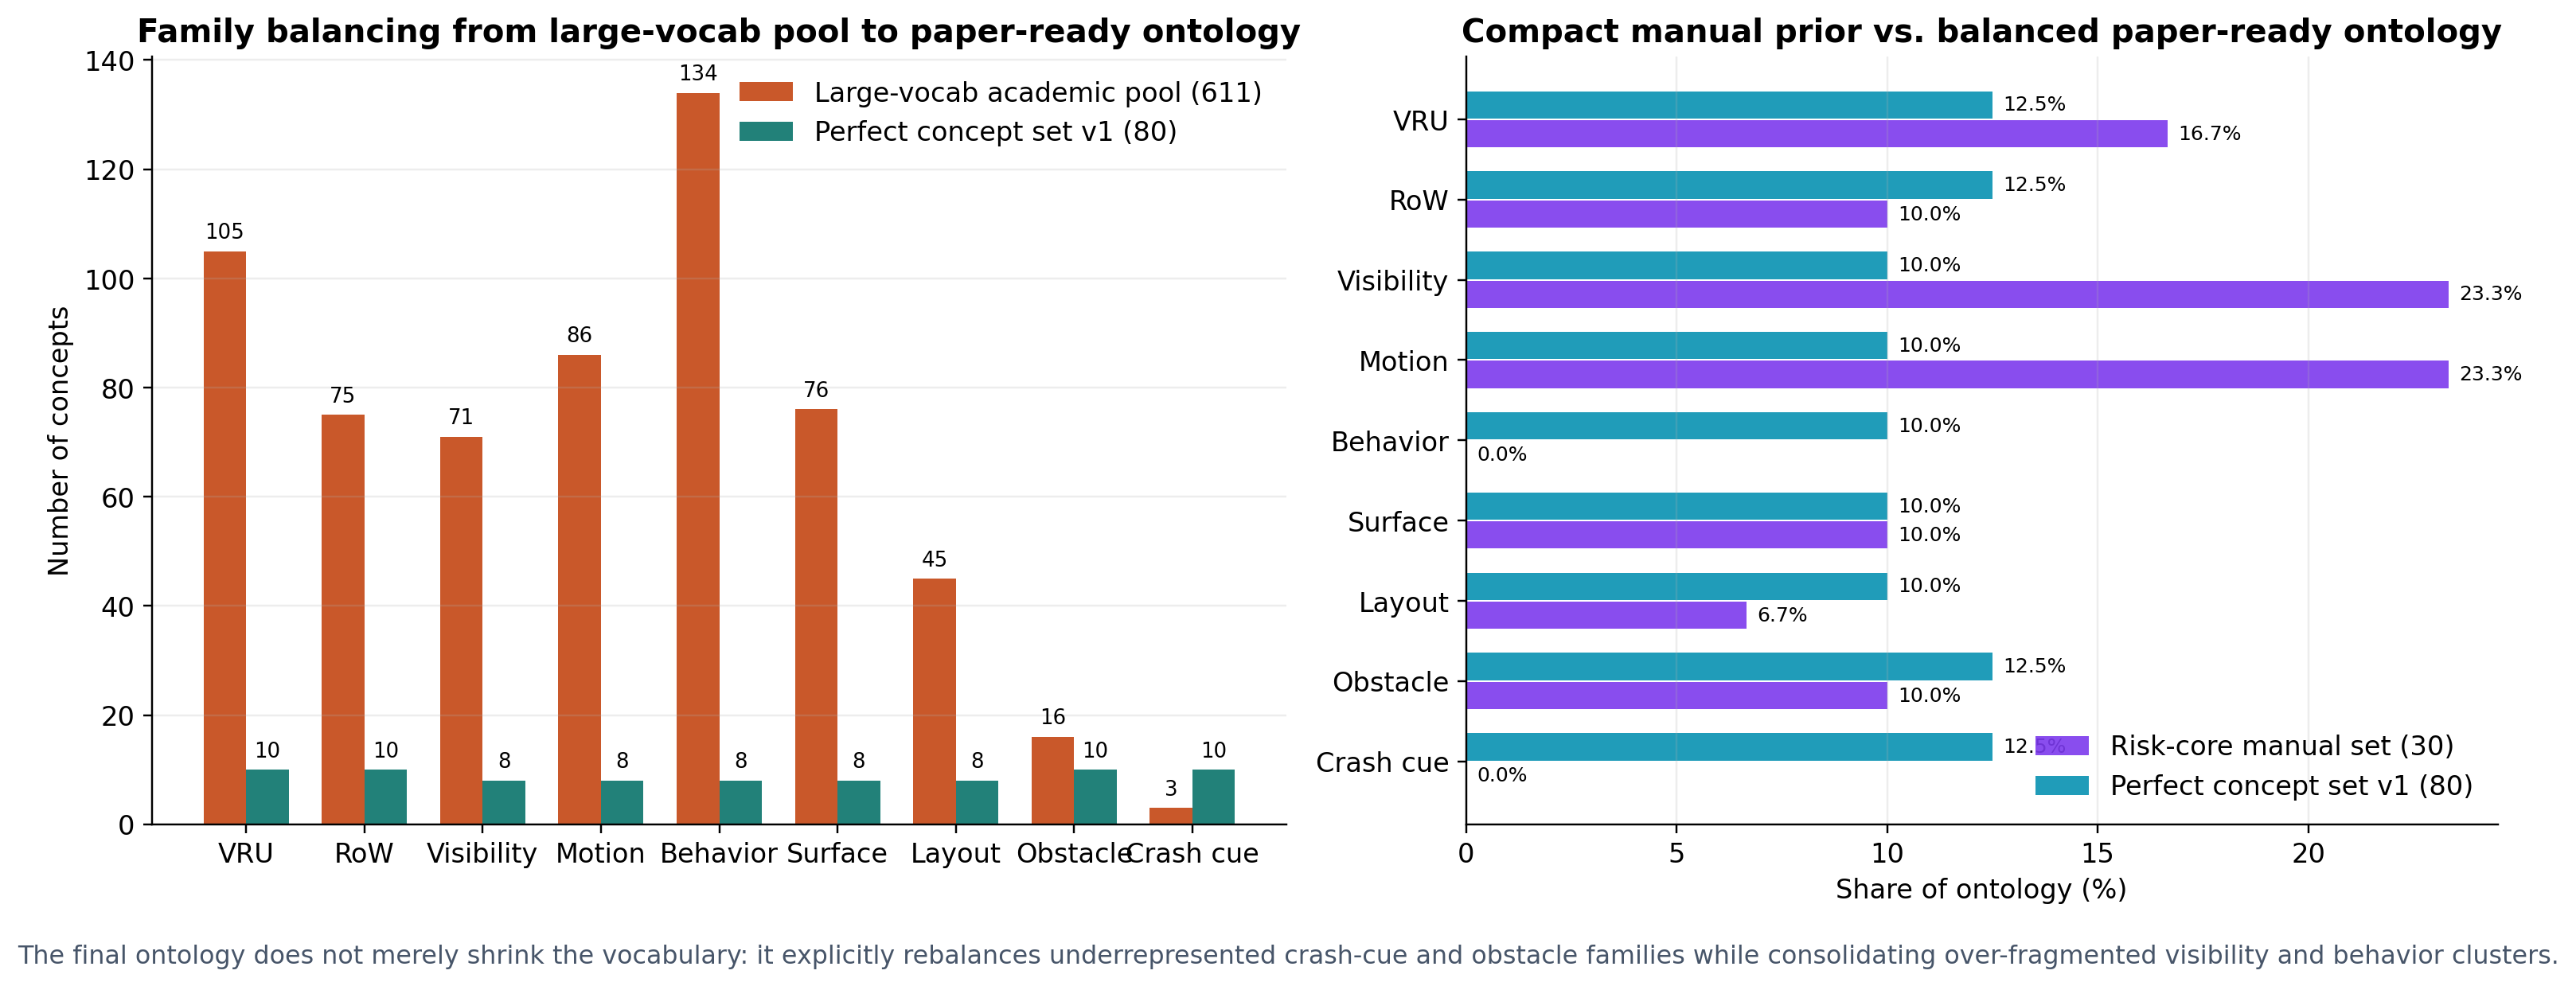
\includegraphics[width=0.98\linewidth]{../figures/insight_fig_concept_family_coverage.pdf}
\caption{[Language-side support evidence] Family coverage in the paper-facing ontology. The polished concept
set deliberately redistributes capacity toward accident-relevant semantic
families, making the ontology easier to audit and more aligned with the target
task than a broad ungoverned phrase pool.}
\label{fig:ontology_family_main}
\end{figure}

\begin{figure*}[t]
\centering
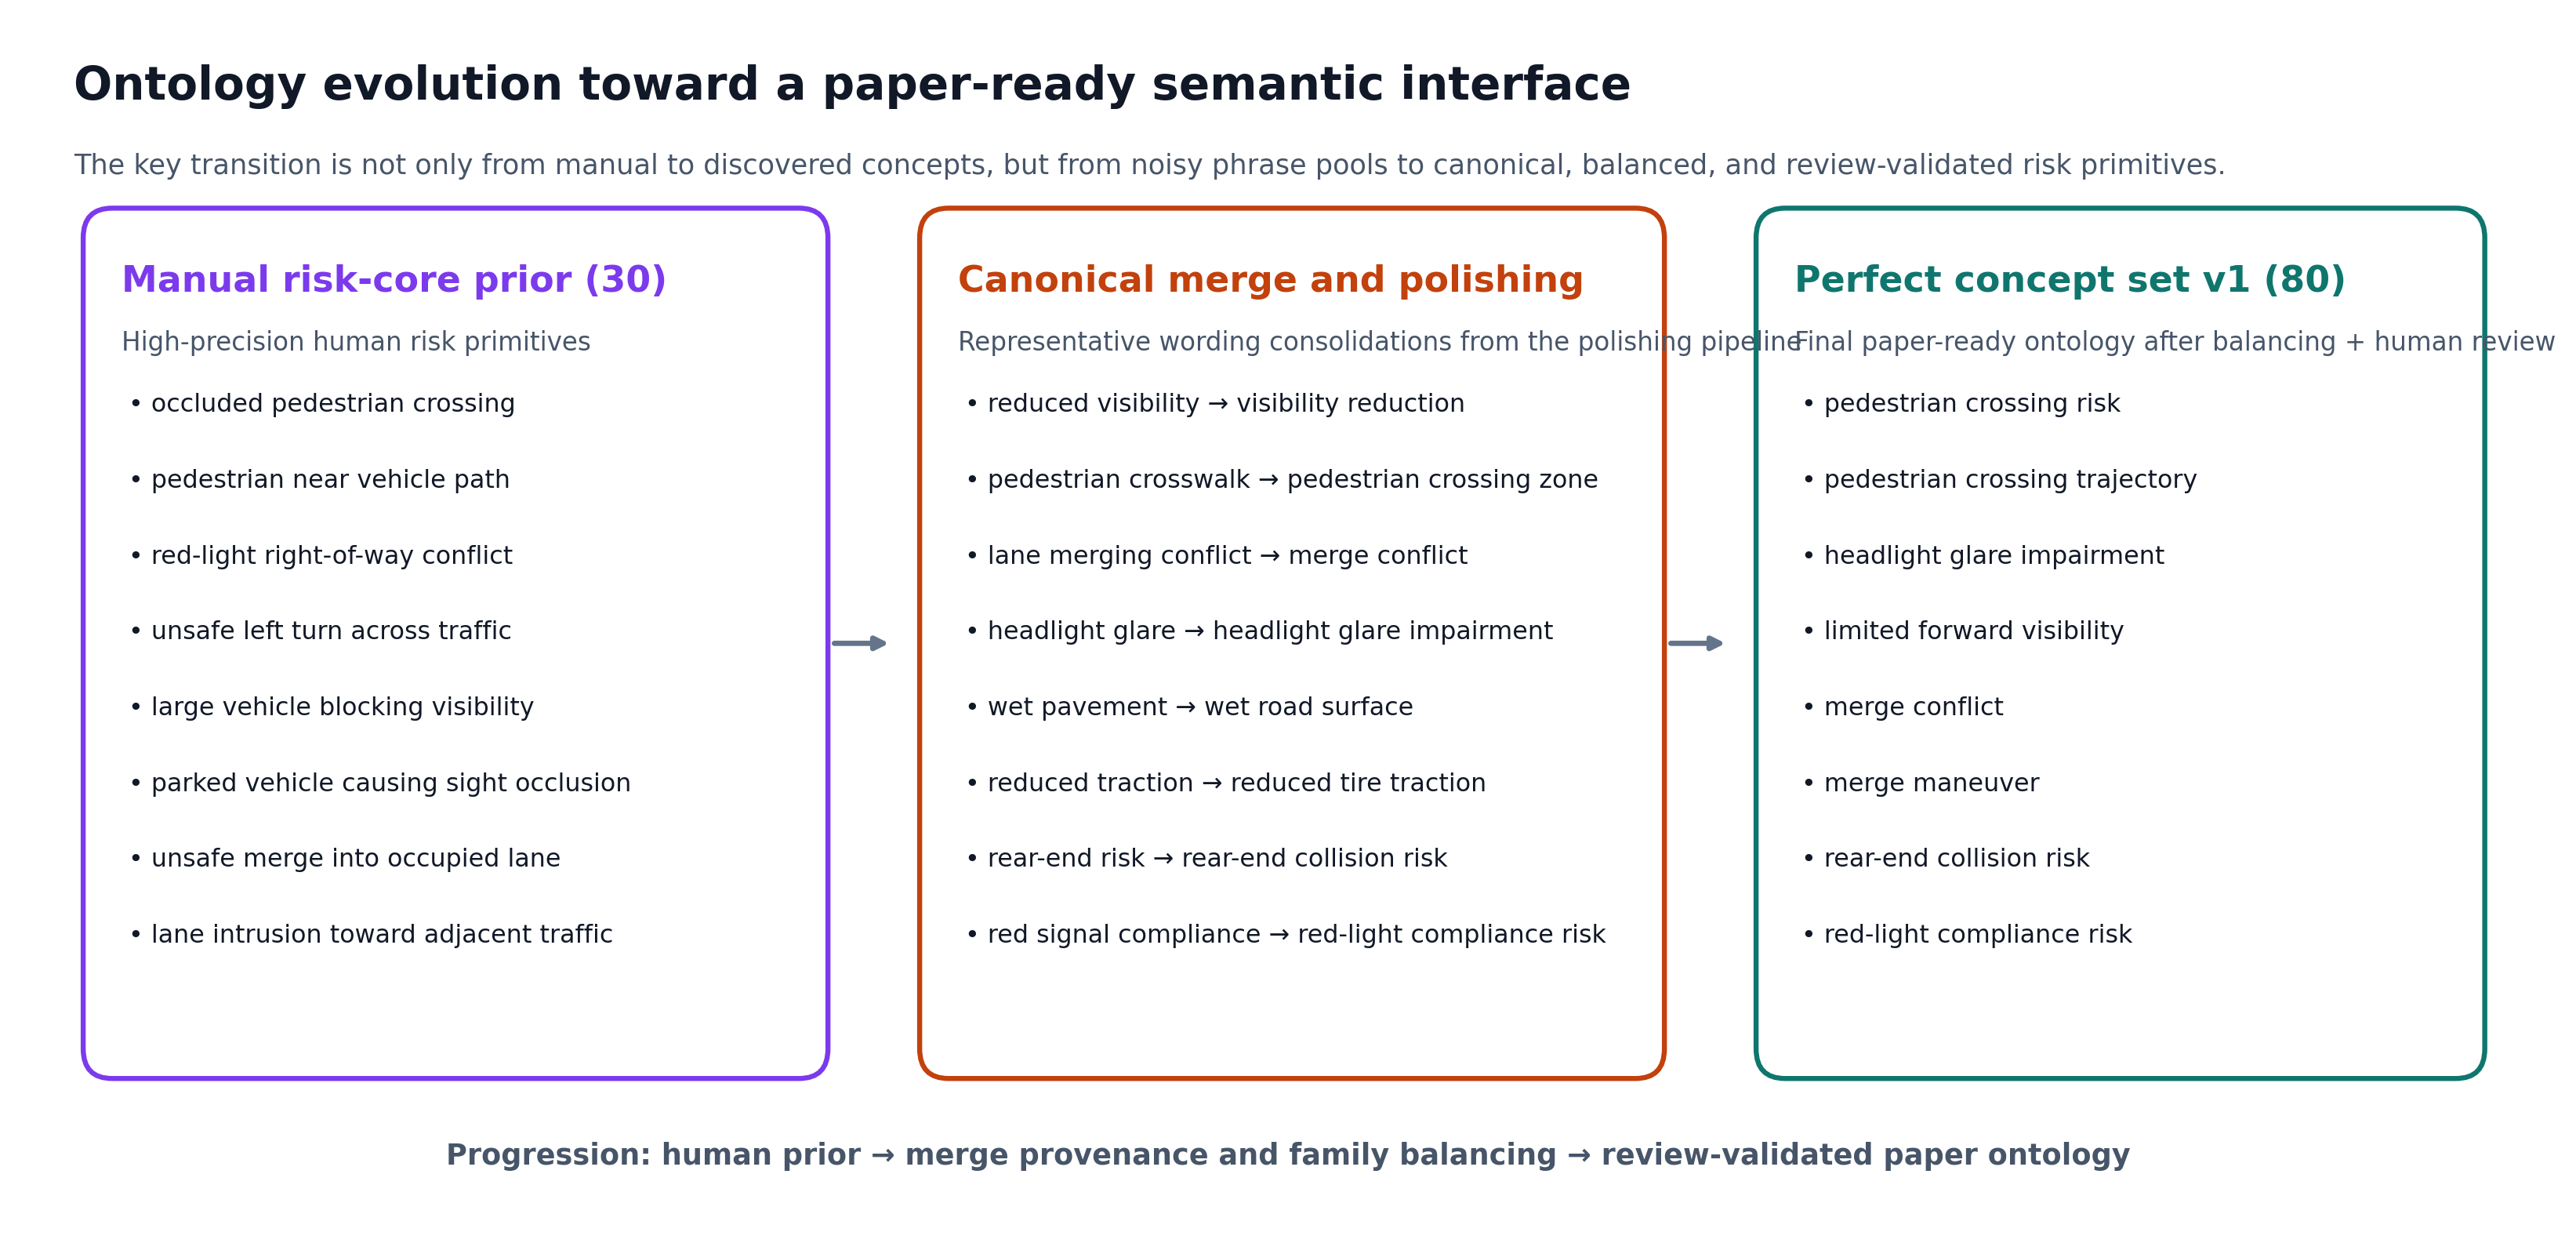
\includegraphics[width=0.98\textwidth]{../figures/insight_fig_concept_evolution.pdf}
\caption{[Language-side support evidence] Ontology evolution toward a paper-ready semantic interface. The
semantic bottleneck is not fixed once and for all: we start from a compact
human prior, consolidate noisy large-vocabulary proposals through canonical
merge and family balancing, and then finalize a reviewed ontology that can be
used consistently in both experiments and paper-facing audits.}
\label{fig:ontology_evolution_main}
\end{figure*}

Figures~\ref{fig:ontology_family_main} and
\ref{fig:ontology_evolution_main} illustrate the kind of evidence we want the
ontology to provide: not only a list of names, but a task-facing semantic
structure whose coverage, merge provenance, and review trajectory can be
inspected quantitatively. This is why ontology design appears as a scientific
variable in Table~\ref{tab:concept_sets} rather than as a hidden prompt choice.

\subsection{Concept-Level Quantitative Evidence}

\begin{table}[t]
\caption{[Mechanism stress evidence] Quantitative semantic-interface
diagnostics from archived DAD
analyses. These diagnostics complement the case studies by quantifying timing
alignment, edit sensitivity, and actor behavior in the archived DAD assets.}
\label{tab:interp_quant}
\centering\scriptsize
\setlength{\tabcolsep}{2.5pt}
\resizebox{\linewidth}{!}{%
\begin{tabular}{p{0.23\linewidth}p{0.14\linewidth}p{0.25\linewidth}p{0.30\linewidth}}
\toprule
Diagnostic & Samples & Main statistic & Reading \\
\midrule
Prediction timing & 39 valid positives & mean lead = 39.41 frames ($\approx$1.97s) & event-aligned timing is measurable before impact \\
Hybrid amplification & 50 edited cases & mean shift = $-2.04$ frames & positive edits can advance alerts in some cases \\
Hybrid amplification & 50 edited cases & earlier / same / later = 14\% / 84\% / 2\% & edit effects are heterogeneous, not universal \\
Zero-baseline edit & 25 edited cases & mean shift = 0.00 frames & null-style edit has no systematic timing effect \\
Top-risk edit & 25 edited cases & mean shift = 0.00 frames & naive top-risk edits alone do not guarantee movement \\
Actor diagnostic & 48 cases & mean actor peak = 0.498 & archived actor outputs are too flat for strong policy claims \\
\bottomrule
\end{tabular}%
}
\end{table}

Table~\ref{tab:interp_quant} records what the archived analyses support
quantitatively: prediction timing can be aligned
to accident onset, positive concept edits can move alerts earlier on a
meaningful subset of cases, and the archived actor branch is too flat for
strong policy claims. These numbers support the paper's current stance: the
semantic interface is architecturally transparent and partially audited, but it
is not yet a finished human-verified concept benchmark or a complete causal
timing proof. That asymmetry is intentional in our presentation: the paper is
strongest as a semantic-interface paper, not as a claim that every downstream
timing component is already equally mature.

\subsection{Ablation and Efficiency}

\begin{table}[t]
\caption{[Controlled support evidence] Component ablation on DAD under a
controlled support protocol. These runs are not the canonical headline
line; their purpose is to
isolate how much the concept interface and its support modules matter under a
shared recipe.}
\label{tab:ablation}
\centering\small
\setlength{\tabcolsep}{4pt}
\resizebox{\linewidth}{!}{%
\begin{tabular}{lccc}
\toprule
Variant & AP$\uparrow$ & mTTA$\uparrow$ & TTA@R80$\uparrow$\\
\midrule
Full \method                  & \textbf{68.84\%} & \textbf{2.42s} & \textbf{3.15s}\\
\quad w/o \caac{} (CBM-only)  & 67.1\% & 1.75s & 2.31s\\
\quad w/o \cgta{}             & 67.8\% & 2.19s & 2.87s\\
\quad w/o \crs{}              & 68.2\% & 2.31s & 3.02s\\
\quad w/o \tsd{}              & 67.5\% & 2.28s & 2.95s\\
\quad w/o \cbm{} (no concepts)& 65.3\% & 1.82s & 2.44s\\
\bottomrule
\end{tabular}%
}
\end{table}

The ablation shows that the semantic interface participates in predictive
behavior, but the DAD mechanism story should still be read with some care and as
mechanism-support rather than headline evidence. Within this controlled support
line, removing the concept bottleneck hurts performance, and removing the
timing consumer or concept-linked temporal modeling also weakens the operating
point. At the same time, our broader three-seed support family for DAD ablations
shows that the no-\cbm{} variant can remain competitive on AP under some matched
support recipes. We therefore avoid the stronger claim that DAD gains are
explained by the concept bottleneck alone. The safer reading is that the
semantic interface, temporal coupling, and training recipe interact, with A3D
providing the cleaner mechanism story and DAD providing the more fragile one.

Archived A3D support ablations point in the same direction but with a cleaner
mechanism profile. In that family, removing the concept bottleneck lowers AP
from $94.75\%$ to $93.47\%$ and mTTA from $4.81$~s to $4.61$~s, while removing
reconstruction lowers AP to $93.38\%$. Removing alignment raises AP to
$96.03\%$, but it simultaneously shortens mTTA to $4.27$~s and TTA@R80 to
$3.70$~s from the full line's $4.44$~s. We therefore read A3D as evidence that
the semantic interface is most convincing as an operating-point design: some
auxiliary terms can trade AP against timing, but removing the bottleneck itself
still weakens the cleaner paper-facing support family.

From an efficiency perspective, \method{} remains in a small-model regime
(about 30M parameters), far below several strong but non-interpretable
alternatives. The practical claim is therefore modest but relevant:
architectural auditability does not require the largest models in the current
literature.

\paragraph{Cross-dataset interpretation.}
Taken together, the results suggest that \method{} is strongest when hazards
develop progressively enough for semantic precursor cues to appear before
impact. This likely explains the stronger A3D behavior. DAD still benefits,
but offers a narrower and noisier early-warning window, so claims there are
fragile support rather than a settled high-confidence mechanism statement.

\subsection{Qualitative Interface Evidence}

\begin{figure*}[t]
  \centering
  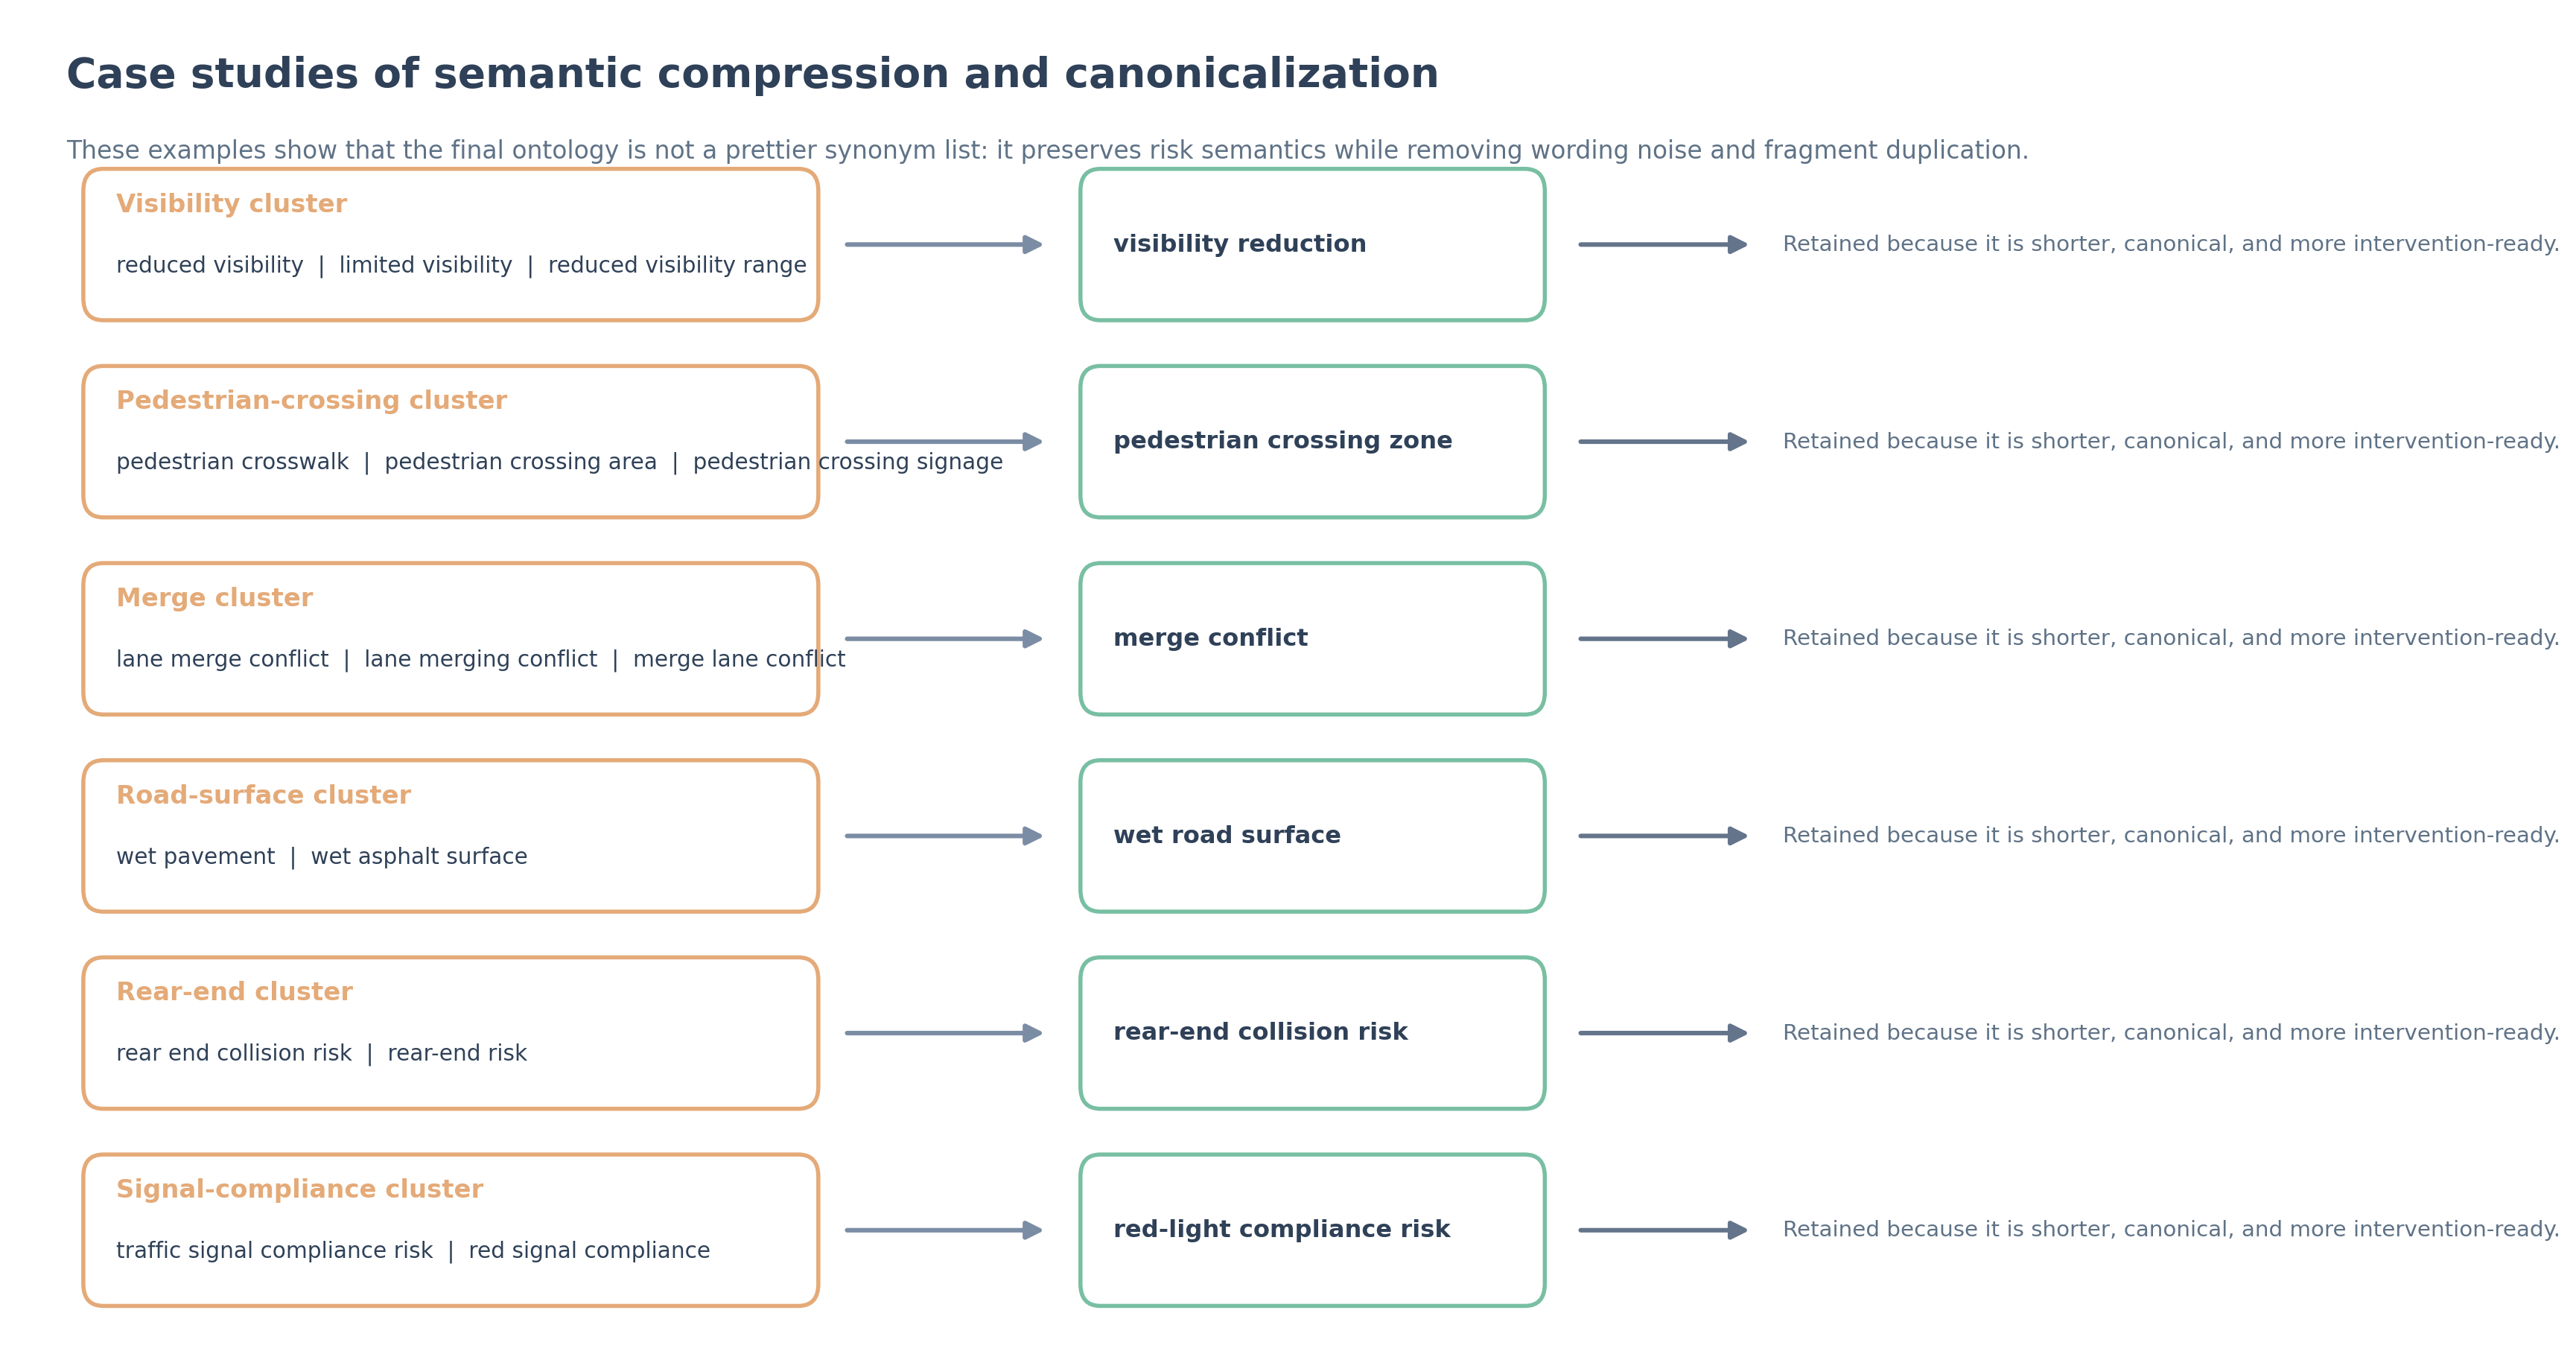
\includegraphics[width=0.985\textwidth]{../figures/insight_fig_concept_case_study.pdf}
  \caption{\textbf{Canonical merge examples from the paper-facing ontology.}
  The final ontology is not just shorter than the raw proposal pool. It
  preserves risk semantics while consolidating wording noise into canonical,
  intervention-ready concepts such as \emph{visibility reduction},
  \emph{pedestrian crossing zone}, and \emph{merge conflict}.}
  \label{fig:concept_case_study_main}
\end{figure*}

Figure~\ref{fig:motivation} already shows the semantic interface in use on a
real crash case, where concept activations and temporal evolution can be read
directly against the scene progression. Figure~\ref{fig:concept_case_study_main}
complements that example from the ontology side by making the canonical merge
policy concrete. Together, these figures show what we mean by a paper-ready
semantic interface: readable at inference time, but also governed as a stable
research artifact rather than as an ad hoc phrase bank.
